\documentclass[english,master]{liumaiex}
% Options are english, swedish, bachelor and master


%=========================================================================%
%
% Add optional packages. Some are almost essential. 
%
%=========================================================================%
\usepackage{amssymb}
\usepackage{amsmath}
\usepackage[dvips]{graphicx}
\usepackage{xcolor}
\usepackage{amsthm}
\usepackage{comment}
\usepackage{parskip}
\usepackage{tikz}
\usepackage{lipsum}
\usepackage{makecell}
\usepackage{pgfplots}
\usepackage{mathtools}
\usepackage{forest}
\usepackage{bm}
\usepackage{float}
\usepackage{subcaption}
\pgfplotsset{compat=1.18}
\usetikzlibrary{calc}

\theoremstyle{plain}
\newtheorem{proposition}{Proposition}[section]
\newtheorem{corollary}[proposition]{Corollary}
\newtheorem{lemma}[proposition]{Lemma}
\newtheorem{theorem}[proposition]{Theorem}
\newtheorem{conjecture}[proposition]{Conjecture}
\theoremstyle{definition}
\newtheorem{definition}[proposition]{Definition}
\newtheorem{example}[proposition]{Example}
\newtheorem{remark}[proposition]{Remark}

\newcommand\todo[1]{\textcolor{red}{#1}}
\DeclareMathOperator{\sgn}{sgn}
\newcommand{\tr}{\text{tr}}
\DeclarePairedDelimiter\ceil{\lceil}{\rceil}
\DeclarePairedDelimiter\floor{\lfloor}{\rfloor}
\newcommand\smalldots{\hbox to 1em{.\hss.\hss.}}

% Define a macro for the position calculation
\newcommand{\dotposition}[1]{
    ({-360/\n * (#1 - 1) + 90}:\radius)
}

\begin{document}


%=========================================================================%
%
% Information to fill-in
%
%=========================================================================%
\title{The title of the thesis}
\author{Erik Jonasson}
\shortauthor{Jonasson}
% If there are several authors, just enter the names separated by comma or 'and'
\publishmonth{June}
\publishyear{2024}
%\city{City} % Has Linköping as default
%\department{Department name} % Has MAI as default
\supervisor*{Hans Lundmark}
% To add another supervisor, just use the command again
\examiner*{Fredrik Andersson} % use a star to add department automatically
% \supervisor also accepts the star format
%\level{G2} % Not needed when bachelor/master is set in options
%\credits{16 hp} % Not needed when bachelor/master is set in options
\regnumber{The number your thesis gets from administrators}
\enkeywords{Keyword 1, keyword 2, etc.}
\svkeywords{Nyckelord 1, nyckelord 2, etc.}
\publishurl{The url to the thesis}
%\pdfauthor{Name} % Needed if name is complex
%\pdftitle{Title} % Needed if title is complex
%\pdfkeywords{Keywords} % Needed if keywords are complex
%\pdfsubject{Subject} % Optional

\maketitle


%=========================================================================%
%
% Introductory part: Abstract, Acknowledgements, etc 
%
%=========================================================================%
\pagenumbering{roman}
\section*{Abstract}

A summary of the thesis, presenting the important results.

\placeenkeywords
\placeenurl

\newpage

% \cleardoublepage
% \begin{otherlanguage*}{swedish}
% \chapter*{Sammanfattning}

% You can write a swedish abstract in this environment to get
% correct (swedish) formatting and hyphenation

% \placesvkeywords
% \placesvurl
% \end{otherlanguage*}

% \chapter*{Acknowledgements}

% Acknowledgements and thanks to people that have helped you.

% \chapter*{Nomenclature}

% The notation you will use in the thesis

\tableofcontents
%\listoffigures
%\listoftables

\newpage



%=========================================================================%
%
% Main part of the thesis
%
%=========================================================================%
\pagenumbering{arabic}

\section{Introduction}

The objective of this thesis is to study the following nonlinear partial differential equation (PDE):
\begin{equation}
	u_{xxt} = -u^2u_{xxx} - 3uu_xu_{xx},
\end{equation}
where $u = u(x, t)$. This equation is obtained by taking the high-frequency limit of the Novikov equation which will be explained in this section. It can be written on a more compact form as
\begin{equation}
	m_t + ((um)_x + 2u_xm) u = 0,\quad m = u_{xx}.
\end{equation}
We will study solutions to this equation on the form,
\begin{equation}
	u(x, t) = \sum_{k = 1}^{N} m_k(t) |x - x_k(t)|.
\end{equation}
Solution on this form gives rise to a system of ordinary differential equations (ODEs). The ODEs are given by
\begin{equation}
	\dot{x}_k = u(x_k)^2, \quad
	\dot{m}_k = -m_ku_x(x_k)u(x_k).
\end{equation}
In the next section a brief historical background will be given and then the high-frequency limit of the Novikov equation and two closely related PDEs will be discussed. After that a brief outline of the thesis will be given.

\subsection{A short history of solitons}

In 1834 John Scott Russell observed a solitary wave in a canal. The wave was created by a boat traveling along the canal. The wave was solitary in that it maintained its shape and speed as it traveled along the canal.

Diederik Johannes Korteweg and Gustav de Vries continued the study of solitary waves and they were the first to derive a partial differential equation (PDE) that describes solitary waves. In 1895 they discovered the now famous Korteweg--de Vries (KdV) equation
\begin{equation}
	u_t + u_{xxx} - 6uu_x = 0,
\end{equation}
that describes solitary waves in shallow water.

It was not until much later in 1965 that Zabusky and Kruskal \cite{Zabusky1965} discovered numerically that the KdV equation has solutions of solitary travelling waves that can interact with each other without changing shape. They called these solitary waves solitons. Solitons have since been studied in many fields such as fluid dynamics, optics, and quantum mechanics.

In 1993\cite{Camassa_1993}, while working on an integrable model of one-dimensional dispersive waves in shallow water Camassa and Holm discovered the first PDE which admit peakon (peaked soliton) solutions. The Camassa--Holm (CH) equation
\begin{equation} \label{eq:CH}
	m_t + (um)_x + u_xm = 0,\quad m = u - u_{xx},
\end{equation}
opened up the door for many other PDEs with peakon solutions. The peakon traveling wave moves at a speed based on its maximum height, at which
it has a sharp peak (jump in derivative). These peakon solutions have the following form
\begin{equation} \label{eq:peakon}
	u(x, t) = \sum_{k = 1}^{N} m_k(t) e^{-|x - x_k(t)|}.
\end{equation}
Later the Degasperis--Procesi (DP) equation
\begin{equation} \label{eq:DP}
	m_t + (um)_x + 2u_xm = 0,\quad m = u - u_{xx}.
\end{equation}
was studied by Degasperis and Procesi in 1999 \cite{Degasperis_1999}. Both the CH and DP equations share similar properties with the Novikov equation. For a more detailed discussion of the peakon equations and their properties, see the comprehensive overview by Lundmark and Szmigielski \cite{Lundmark_2022}.

This brings us back to the Novikov equation
\begin{equation} \label{eq:Novikov_high_freq}
	m_t + ((um)_x + 2u_xm) u = 0,\quad m = u - u_{xx}.
\end{equation}
It was discovered by Vladimir Novikov in a classification of cubically nonlinear PDEs admitting infinitely many symmetries \cite{Novikov_2009}, with Hone and Wang \cite{Hone2008} later providing a Lax pair for it. Lax pairs will be discussed in more detail later in the thesis.

\subsection{High-frequency limit}

As mentioned at the start the focus of the thesis is on the high-frequency limit of the Novikov equation. The high-frequency limit is obtained by substitution of $x \mapsto \epsilon x$, $t \mapsto \epsilon t$, $m \mapsto -\epsilon^{-2} m$, and letting $\epsilon \rightarrow 0$. This limit gives the high-frequency Novikov equation \eqref{eq:Novikov_high_freq}.

Both the CH and DP equations have been studied in the high-frequency limit.  The high frequency limit of the Camassa--Holm equation yields the Hunter--Saxton equation \cite{HunterSaxton_1991,HunterZheng1994} for nematic liquid crystals. The high frequency limit of the Degasperis--Procesi equation yields the derivative Burgers equation \cite{Kohlenberg_2007, Lundmark_2008}.  The only difference between all three of the original equations and their respective high-frequency limit is that $m = u_{xx}$ instead of $m = u - u_{xx}$.

\todo{Write as can be seen in this table:}
\begin{center}
  \begin{tabular}{l|c|c}
    & $m=u-u_{xx}$ & $m=u_{xx}$ \\
    \hline
    $m_t + (um)_x + u_xm = 0$ 
	& \multicolumn{1}{l|}{Camassa--Holm} & \multicolumn{1}{l}{Hunter--Saxton} \\
    \hline
    $m_t + (um)_x + 2u_xm = 0$ 
	& \multicolumn{1}{l|}{Degasperis--Procesi} & \multicolumn{1}{l}{Derivative Burgers} \\
    \hline
    $m_t + ((um)_x + 2u_xm)u = 0$ 
	& \multicolumn{1}{l|}{Novikov} & \multicolumn{1}{l}{HF Novikov} \\
  \end{tabular}
\end{center}

All three high-frequency limits also admits piecewise linear solutions on the following form
\begin{equation} \label{eq:linear_peakon}
	u(x, t) = \sum_{k = 1}^{N} m_k(t) |x - x_k(t)|.
\end{equation}
For the HF Novikov equation the time derivative of $x_k$ and $m_k$ will be governed by the following ODEs
\begin{equation} \label{eq:peakon_odes}
\dot{x}_k = u(x_k)^2, \quad
\dot{m}_k = -m_ku_x(x_k)u(x_k).
\end{equation}
Dots denote $\frac{d}{dt}$ as usual. $u(x_k)$ and $u(x = x_k,t)$ is given by
\begin{align}
	u(x_k) &= \sum_{i = 1}^{N} m_i(t) |x_k - x_i(t)|, \\
	u_x(x_k) &= \sum_{i = 1}^{N} m_i(t) \sgn(x_k - x_i).
\end{align}
The $u_x$ isn't defined at $x = x_i$ but we define it to be the average $\langle u_x(x_i) \rangle$ of the left and right limits and we will see that this is consistent with the PDE.  See Appendix (\ref{sec:DerivationODE}) for the proof that the HF Novikov equation admits piecewise linear solutions on the form of equation \eqref{eq:linear_peakon} and that the ODE-system is compatible with the PDE.

The peakon equations and their respective high-frequency limits share many similarities. The ODEs for both equations share the same form, but the $u(x_k)$ and $u_x(x_k)$ are different. Both the regular and HF Novikov equations only have $x_i$'s that increase due to the $u(x_k)^2$ term in the ODEs.
\begin{center}
  \begin{tabular}{l|c|c}
    & $u=\sum_{i=1}^n m_i e^{-|x-x_i|}$ & $u=\sum_{i=1}^n m_i |x-x_i|$ \\[3pt]
    \hline
    \makecell[l]{
	$\begin{aligned}
		\dot{x}_i &= u(x_k),\\
		\dot{m}_i &= -\phantom{2}m_i u_x(m_i)
	\end{aligned}$}
	& \multicolumn{1}{l|}{Camassa--Holm} & \multicolumn{1}{l}{Hunter--Saxton} \\
    \hline
    \makecell[l]{
	$\begin{aligned}
		\dot{x}_i &= u(x_k),\\
		\dot{m}_i &= -2m_i u_x(m_i)
	\end{aligned}$}
	& \multicolumn{1}{l|}{Degasperis--Procesi} & \multicolumn{1}{l}{Derivative Burgers} \\
    \hline
    \makecell[l]{
	$\begin{aligned}
		\dot{x}_i &= u(x_k)^2,\\
		\dot{m}_i &= -\phantom{2}m_i u_x(m_i) u(x_i)
	\end{aligned}$}
	& \multicolumn{1}{l|}{Novikov} & \multicolumn{1}{l}{HF Novikov} \\
  \end{tabular}
\end{center}

\subsection{Outline}

The initial objective of this thesis was to solve the HF Novikov equation explicitly for any $N$. However, it was found that solving the equation presents significant challenges and the solutions method used for similar equations such as the derivative Burgers equation and the Novikov equation did not work. The thesis will instead focus on other aspects of the HF Novikov equation.

In the next section of the thesis there will be a detailed solution for the case when $N = 2$. The solution will be given for two cases, both the regular and a periodic case which will be discussed in the next section. For higher values of $N$ a numerical analysis will be given in the third section. Then the Hamiltonian structure of the HF Novikov equation will be discuss in section four.

After that in the sections that follow we will examine the constants of motion for the HF Novikov equation. First a short survey of the constants of motion discovered by direct search will be given. Then a more systematic approach will be taken to find the constants of motion for the HF Novikov equation. Next a short theorem of the constants of motion for a generalized system of ODEs will be given. It connects the constant of motion of the HF Novikov equation to the regular Novikov equation. After that the Lax pair will be discussed and the constants of motion derived from it. The thesis will conclude with appendices that provide additional mathematical proofs and verifications.

\section{Solution for N = 2}

For $N = 1$, the solution to the HF Novikov equation is trivial since $u(x_k) = 0$. Therefore, both $\dot{x}_k$ and $\dot{m}_k$ are equal to zero, resulting in a constant solution. For the more interesting case when $N = 2$, we will give a detailed solution to the system of ODEs for the HF Novikov equation. We will also address the periodic case for $N = 2$.

\subsection{HF Novikov equation}
For $N = 2$ the system of ODEs is given by
\begin{equation}
\begin{aligned}
	\dot{x}_k &= u(x_k)^2, \\
	\dot{m}_k &= -m_k u_x(x_k)u(x_k).
\end{aligned}
\end{equation}
The assumption that $x_1 < \cdots < x_N$ can be made without loss of generality. For $N = 1$, the solution is trivial since $u(x_k) = 0$, which appears in both $\dot{x}_k$ and $\dot{m}_k$, so both $\dot{x}_k$ and $\dot{m}_k$ are equal to zero and the solution for is constant. For the more interesting case when $N = 2$ we get the following system of ODEs from equation \eqref{eq:peakon_odes}:
%
\begin{align}
	\dot{x}_1 & = m_2^2 (x_2 - x_1)^2, \\
	\dot{x}_2 & = m_1^2 (x_2 - x_1)^2, \\
	\dot{m}_1 & = m_1 m_2^2(x_2 - x_1),  \\
	\dot{m}_2 & = -m_1^2 m_2(x_2 - x_1).
\end{align}
%
We will also assume that $m_k \neq 0$ since in the case where it is zero it will remain identically zero.
%
To solve this system, we first identify two conserved quantities
\begin{align}
	\label{eq:solution_2N_M}
	M &= m_1^2 + m_2^2, \\
	\label{eq:solution_2N_K}
	K &= m_1m_2(x_2 - x_1).
\end{align}
%
We show that these quantities are conserved by making sure that their time derivatives are zero
\begin{equation}
\begin{aligned}
	(m_1^2 + m_2^2)_t 
	&= 2m_1\dot{m}_1 + 2m_2\dot{m}_2 \\
	&= 2m_1^2m_2^2(x_2 - x_1) - 2m_1^2m_2^2(x_2 - x_1) = 0,
\end{aligned}
\end{equation}
\begin{equation}
\begin{aligned}
	(m_1m_2&(x_2 - x_1))_t \\
	&= \dot{m}_1m_2(x_2 - x_1) + m_1\dot{m}_2(x_2 - x_1)
	- m_1m_2\dot{x}_1 + m_1m_2\dot{x}_2 \\
	&=\phantom{-} m_1m_2^3(x_2 - x_1)^2 - m_1^3m_2(x_2 - x_1)^2 \\
	&\phantom{=}- m_1m_2^3(x_2 - x_1)^2 + m_1^3m_2(x_2 - x_1)^2 \\
	&=0. \\
\end{aligned}
\end{equation}
%
Leveraging these conserved quantities, we derive expressions for $\dot{m}_1$ and $\dot{m}_2$:
\begin{equation}
\begin{aligned}
	\dot{m}_1 = \phantom{-}m_2K, \\
	\dot{m}_2 = -m_1K.
\end{aligned}
\end{equation}
%
The solutions to these equations take the form
\begin{equation}
\begin{aligned}
	m_1 &= \sqrt{M} \sin(Kt + \phi), \\
	m_2 &= \sqrt{M} \cos(Kt + \phi).
\end{aligned}
\end{equation}
%
Now we can solve for $\dot{x}_1$ and $\dot{x}_2$:
\begin{align}
	\dot{x}_1m_1^2 = m_1^2m_2^2(x_2 - x_1)^2 = K^2 \\
	\implies
	\dot{x}_1 = \frac{K^2}{m_1^2} = \frac{K^2}{M\sin^2(Kt + \phi)}, \\
	\dot{x}_2m_2^2 = m_1^2m_2^2(x_2 - x_1)^2 = K^2 \\
	\implies
	\dot{x}_2 = \frac{K^2}{m_2^2} = \frac{K^2}{M\cos^2(Kt + \phi)}.
\end{align}
%
Integration yields the positions:
\begin{equation}
\begin{aligned}
	x_1 = -\frac{K}{M}\cot(Kt + \phi) + C,\\
	x_2 = \phantom{-}\frac{K}{M}\tan(Kt + \phi) - D.
\end{aligned}
\end{equation}
%
The $K$ quantity implies that $D = -C$:
\begin{equation}
\begin{aligned}
	K &= m_1m_2(x_2 - x_1) \\
	&= M \sin(Kt + \phi) \cos(Kt + \phi) \\
	& \qquad \Big( \frac{K}{M} \Big(\frac{\sin(Kt + \phi)}{\cos(Kt + \phi)} +
	\frac{\cos(Kt + \phi)}{\sin(Kt + \phi)}\Big) - D - C \Big) \\
	&= K(\sin^2(Kt + \phi) + \cos^2(Kt + \phi)) \\
	& \qquad - M \sin(Kt + \phi) \cos(Kt + \phi)(C + D) \\
	&= K - M \sin(Kt + \phi) \cos(Kt + \phi)(C + D).
\end{aligned}
\end{equation}
%
Since it has to hold for all $t$, we get that $C + D = 0$. The constant $C$ is determined by the inital conditions
\begin{equation}
	C = \frac{m_2(0)^2 x_2(0) + m_1(0)^2 x_1(0)}{M}.
\end{equation}
In conclusion the piecewise linear solution looks like this:
\begin{align}
	u(x, t) &= m_1|x - x_1| + m_2|x - x_2|, \\
	m_1 &= \phantom{-}\sqrt{M} \sin(Kt + \phi), \\
	m_2 &= \phantom{-}\sqrt{M} \cos(Kt + \phi), \\
	x_1 &= -\frac{K}{M}\cot(Kt + \phi) + C, \\
	x_2 &= \phantom{-}\frac{K}{M}\tan(Kt + \phi) + C.
\end{align}
%
There are four constants $M$, $K$, $\phi$ and $C$, which is to be expected since there are four initial quantities, $m_1(0)$, $m_2(0)$, $x_1(0)$ and $x_2(0)$. We made the assumption that $x_1 < x_2$, will be valid for all $t$.
\begin{equation}
\begin{aligned}
	x_2 - x_1 
	&= \frac{K}{M}(\tan(Kt + \phi) + \cot(Kt + \phi)) \\
	&= \frac{K}{M}\frac{2}{\sin(2Kt + 2\phi)}
\end{aligned}
\end{equation}
The solution is valid only for a finite time, since $x_2$ will go to infinity in a finite time. As $x_2$ goes to infinity, $u(x,t)$ will go to
\begin{equation}
\begin{aligned}
	\lim_{x_2 \to \infty} u(x, t)
	= \lim_{x_2 \to \infty} m_1|x - x_1| &+ \lim_{x_2 \to \infty} m_2|x - x_2| \\
	= m_1|x - C| &+ \lim_{x_2 \to \infty} m_2 x_2 \\
	= m_1|x - C| &+ \lim_{x_2 \to \infty} \frac{K}{\sqrt{M}} \sin(Kt + \phi) \\
	&+ \lim_{x_2 \to \infty} \sqrt{M} \cos(Kt + \phi) C.
\end{aligned}
\end{equation}
Here we have that
\begin{equation}
	x_2 = \frac{K}{M}\tan(Kt + \phi) + C \rightarrow \infty \implies 
		\begin{cases} 
			\sin(K t + \phi) \rightarrow 1 \\
			\cos(K t + \phi) \rightarrow 0
		\end{cases},
\end{equation}
thus the limit of $u(x,t)$ as $x_2$ goes to infinity is
\begin{equation}
	m_1|x - C| + \frac{K}{\sqrt{M}}
\end{equation}
%
It is possible to create a new system from the old one that will conserve the constants of motion as well as keep $\dot{u}(x, t)$ continuous. We define the new system by keeping $x_1$ and $m_1$ as they are and setting $x_2$ to be $-\infty$ and keeping $m_2$ equal to $0$. The difference now is that $x_2$ will not always be greater than $x_1$. With this genealization of the solutions the real axis can be thought of as a circle and when one of the $x_i$'s reaches $\infty$ it comes back at $-\infty$. The solution for the new system is then given by the same equations as before. Thus it seems possible to create a weak solution for $u(x,t)$ that is valid for all time as long as we define $u(x, t)$ at the points where $x_i$ goes to $\infty$ to be the limit of the solution as $x_i$ goes to $\infty$.

Looking at the asymptotic behavior of the solution we see that $m_1$ always goes to $\pm M$ as $m_2$ goes to zero. The asymptoticics can be visualized by looking at how the momenta move on the circle with radius $M_1$:
\begin{center}
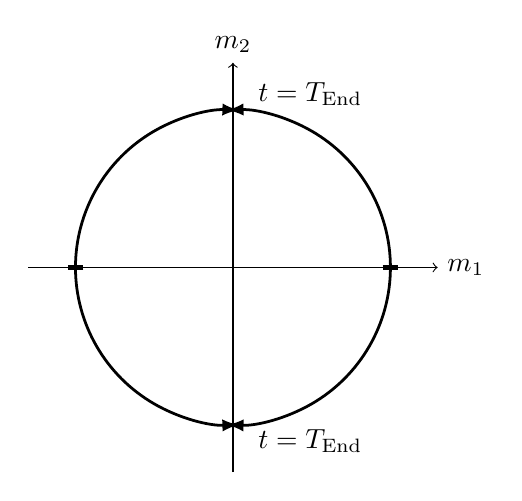
\begin{tikzpicture}[scale=2]
    % Draw the coordinate axes
    \draw[->] (-1.3,0) -- (1.3,0) node[right] {$m_1$};
    \draw[->] (0,-1.3) -- (0,1.3) node[above] {$m_2$};
    \draw[line width=2pt] (0.95,0) -- (1.05, 0);
    \draw[line width=2pt] (-0.95,0) -- (-1.05, 0);
    
    % Draw the circle
    % \draw (0,0) circle (1cm);

    % \node[right] at (1, 0.2) {$t=T_{Start}$};
    \node[right] at (0.1, 1.1) {$t=T_{\text{End}}$};
    \node[right] at (0.1, -1.1) {$t=T_{\text{End}}$};


    % Add arrows along the circle pointing to the top
    \draw[->, >=latex, line width=1pt] (0:1) arc[start angle=0,end angle=92,radius=1cm];
    \draw[->, >=latex, line width=1pt] (0:-1) arc[start angle=180,end angle=88,radius=1cm];
    \draw[->, >=latex, line width=1pt] (0:1) arc[start angle=0,end angle=-92,radius=1cm];
    \draw[->, >=latex, line width=1pt] (0:-1) arc[start angle=-180,end angle=-88,radius=1cm];
\end{tikzpicture}
\end{center}
Here $T_{\text{End}}$ is the time when $x_2$ goes to infinity. Which $T_{\text{End}}$ it goes to depends on the initial conditions. The continuatin of the solution can then be visualized by continuing travelling along the circle in the same direction as before.

While the $x_2$ term goes to infinity the $x_1$ term goes to $C$. For the continuation of the solution it is always true that the smaller $x_i$ will go to $C$. Here is a graph of the values of $x_1$ and $x_2$ over time:

\begin{center}
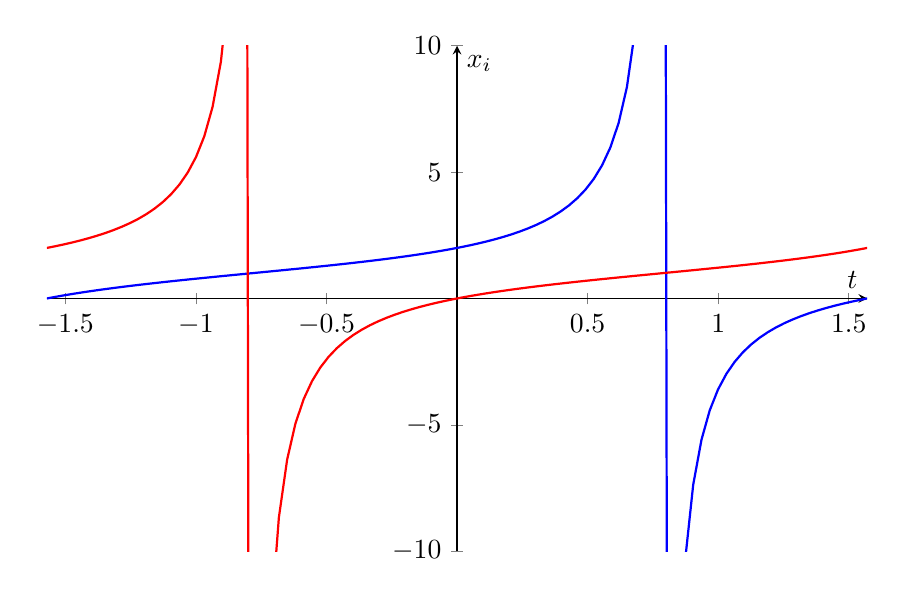
\begin{tikzpicture}
    \begin{axis}[
        xlabel={$t$},
        ylabel={$x_i$},
        domain=-pi/2:pi/2,
        samples=100,
		ymin=-10, ymax=10,
        % grid=both,
        width=12cm,
        height=8cm,
		axis x line=middle, % Optional: centers x-axis
        axis y line=middle, % Optional: centers y-axis
    ]
        \addplot[blue, thick] {tan(deg(x + pi/4)) + 1};
        \addplot[red, thick] {-cot(deg(x + pi/4)) + 1};
    \end{axis}
\end{tikzpicture}
\end{center}

\subsection{Periodic HF Novikov equation}

The $u$ and $u_x$ functions have been adjusted to for the periodic boundary conditions
\begin{equation} \label{eq:periodic_ansatz}
\begin{aligned}
	u(x, t) &= \sum_{k = 1}^{N} m_k(t) |[x - x_k(t) - L]_{2L} - L|, \\
	u_x(x, t) &= \sum_{k = 1}^{N} m_k(t) \sgn([x - x_k(t) - L]_{2L} - L),
\end{aligned}
\end{equation}
where
\begin{equation}
	[x]_{2L} = x - 2L\floor*{\frac{x}{2L}}.
\end{equation}
%
Here is an example of how the function $u$ can look like in black with its two contributing terms in red and blue
\begin{center}
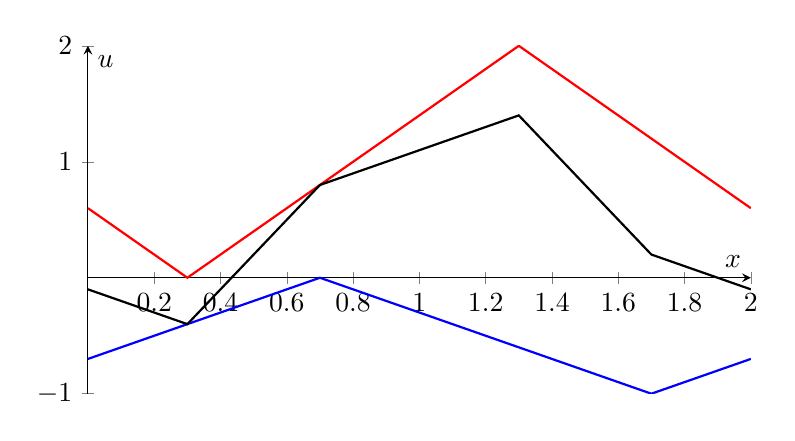
\begin{tikzpicture}
    \begin{axis}[
        xlabel={$x$},
        ylabel={$u$},
		axis x line=center,
		axis y line=center,
        domain=0:2,
        samples=21,
		ymin=-1, ymax=2,
		xmin=0, xmax=2,
        % grid=both,
        width=10cm,
        height=6cm,
    ]
		\addplot[thick, red] {2 * abs(mod(abs(x - 0.3 - 1), 2) - 1)};
        \addplot[thick, blue] {-1 * abs(mod(abs(x - 0.7 - 1), 2) - 1)};
        \addplot[thick, black] {
			+2 * abs(mod(abs(x - 0.3 - 1), 2) - 1)
			-1 * abs(mod(abs(x - 0.7 - 1), 2) - 1)
		};
    \end{axis}
\end{tikzpicture}
\end{center}
%
This leads to the following ODEs for the peakon positions and momenta
%
\begin{align}
	\dot{x}_1 & = m_2^2 ([x_2 - x_1 - L]_{2L} - L)^2, \\
	\dot{x}_2 & = m_1^2 ([x_2 - x_1 - L]_{2L} - L)^2, \\
	\dot{m}_1 & = m_1 m_2^2([x_2 - x_1 - L]_{2L} - L),  \\
	\dot{m}_2 & = -m_1^2 m_2([x_2 - x_1 - L]_{2L} - L).
\end{align}
%
To solve this system, we first identify two conserved quantities
\begin{align}
	M &= m_1^2 + m_2^2, \\
	K &= m_1m_2|[x_2 - x_1 - L]_{2L} - L|.
\end{align}
%
We show that these quantities are conserved by making sure that their time derivatives are zero
\begin{equation}
\begin{aligned}
	(m_1^2 + m_2^2)_t 
	&= 2m_1\dot{m}_1 + 2m_2\dot{m}_2 \\
	&= (2m_1^2m_2^2 - 2m_1^2m_2^2)([x_2 - x_1 - L]_{2L} - L) = 0,
\end{aligned}
\end{equation}
\begin{equation}
\begin{aligned}
	(m_1m_2&|[x_2 - x_1 - L]_{2L} - L|)_t \\
	&= (\dot{m}_1m_2 + m_1\dot{m}_2)|[x_2 - x_1 - L]_{2L} - L| \\
	&+ m_1m_2(\dot{x}_2 - \dot{x}_1)\sgn([x_2 - x_1 - L]_{2L} - L) \\
	&=(m_1m_2^3 - m_1^3m_2 + m_1^3m_2 - m_1m_2^3)\\
	&\phantom{=}|[x_2 - x_1 - L]_{2L} - L|([x_2 - x_1 - L]_{2L} - L) =0. \\
\end{aligned}
\end{equation}
%
Leveraging these conserved quantities, we derive expressions for $\dot{m}_1$ and $\dot{m}_2$:
\begin{equation}
\begin{aligned}
	\dot{m}_1 = \phantom{-}m_2K \sgn([x_2 - x_1 - L]_{2L} - L), \\
	\dot{m}_2 = -m_1K \sgn([x_2 - x_1 - L]_{2L} - L).
\end{aligned}
\end{equation}
%
Let
\begin{equation}
	S(t_0) = \sgn([x_2 - x_1 - L]_{2L} - L).
\end{equation}
The $S(t_0)$ function can only take on the values $-1$, $0$, or $1$. For a momement let's assume that the $S(t_0)$ is equal to $1$. Then we can solve the ODEs for $m_1$ and $m_2$ around $t_0$
\begin{equation}
\begin{aligned}
	m_1 &= \sqrt{M} \sin(K t + \phi), \\
	m_2 &= \sqrt{M} \cos(K t + \phi), \\
	\phi &= \text{atan2}(m_1(0),m_2(0)).
\end{aligned}
\end{equation}
The solution functions for $m_1$ and $m_2$ are the same as for the non periodic case as long as assumption that $S(t_0) = 1$. The same is true for the $x_1$ and $x_2$ solution functions since
\begin{align}
	\dot{x}_1m_1^2 = m_1^2m_2^2(x_2 - x_1)^2 = K^2 \\
	\implies
	\dot{x}_1 = \frac{K^2}{m_1^2} = \frac{K^2}{M\sin^2(Kt + \phi)}, \\
	\dot{x}_2m_2^2 = m_1^2m_2^2(x_2 - x_1)^2 = K^2 \\
	\implies
	\dot{x}_2 = \frac{K^2}{m_2^2} = \frac{K^2}{M\cos^2(Kt + \phi)}.
\end{align}
%
And just as before we can integrate these equations to get the positions
\begin{equation}
\begin{aligned}
	x_1 = -\frac{K}{M}\cot(Kt + \phi) + C,\\
	x_2 = \phantom{-}\frac{K}{M}\tan(Kt + \phi) - D,
\end{aligned}
\end{equation}
which results in the same solution as for the non periodic case
\begin{align}
	m_1 &= \sqrt{M} \sin(K t + \phi), \\
	m_2 &= \sqrt{M} \cos(K t + \phi), \\
	x_1 &= -\frac{K}{M}\cot(Kt + \phi) + C,\\
	x_2 &= \phantom{-}\frac{K}{M}\tan(Kt + \phi) + D,
\end{align}
with the only difference that $C$ and $D$ doesn't not need to be equal. The constants $C$ and $D$ are determined by the inital conditions
\begin{equation}
\begin{aligned}
	C &= x_1(0) + \frac{K}{M}\frac{m_2(0)}{m_1{0}}, \\
	D &= x_2(0) - \frac{K}{M}\frac{m_1(0)}{m_2{0}}.
\end{aligned}
\end{equation}
It's important to note that since we used that $S(t_0) = 1$ here we only got a local solution. The $S(t_0)$ function will change sign if the $x_2$ and $x_1$ swap places in the expression for $S(t_0)$
\begin{equation}
\begin{aligned}
	\sgn([x_1 - x_2 - L]_{2L} - L) =& \sgn([x_2 - x_1 - L + 2L]_{2L} - L)  \\
	=& \sgn([-(x_2 - x_1 - L)]_{2L} - L) \\
	=& \sgn(-[x_1 - x_2 - L]_{2L} + L) \\
	=& -S(t_0).
\end{aligned}
\end{equation} 
This tells us that the solution for when $S(t_0) = -1$ can be obtained by swapping the solution functions for $m_1$ and $m_2$ as well as for $x_1$ and $x_2$.
\\ \\
For the case where $S(t_0) = 0$ we have that $m_1$ and $m_2$ are constant and from the ODEs for $x_1$ and $x_2$ we see that the time derivative of $x_1$ and $x_2$ will be the same only if $m_1 = m_2$. This means that if $S(t_0) = 0$ and $m_1(t_0) = m_2(t_0)$ is going to be constant and $x_1$ and $x_2$ will both travel with constant speed with a distance of $L$ between them. In the case where $S(t_0)$ and $m_1(t_0) \neq m_2(t_0)$ the solution will be only be valid for $t = t_0$. At any other $t$ close to $t_0$ the $S(t)$ function will be either $-1$ or $1$.
\\ \\
As soon as the local solution becomes invalid it's possible to continue the solution by creating a new solution with new values for $C$, $D$, $\phi$. Both $M$ and $K$ are will be conserved for the continuation of the solution. The non-periodic solution can be obtained by letting $L \rightarrow \infty$, since that will make the periodic boundary conditions irrelevant.

\section{Numerical analysis} \label{sec:Numerical}

\todo{Numerical simulations have been done. Just need to decide what's worth mentioning. Maybe confimation of the N=2 solution, confimation of the constants of motion, collisions, periodic?}

Both in the non periodic and periodic cases the numerical simulations are consistent with the analytical solution for $N = 2$ and the constants of motion for larger $N$.

\subsection{HF Novikov equation}

First we will look at the graph of $x_i$ and $m_i$ for $N = 3$.
\begin{figure}[H]
	\begin{subfigure}{0.44\textwidth}
		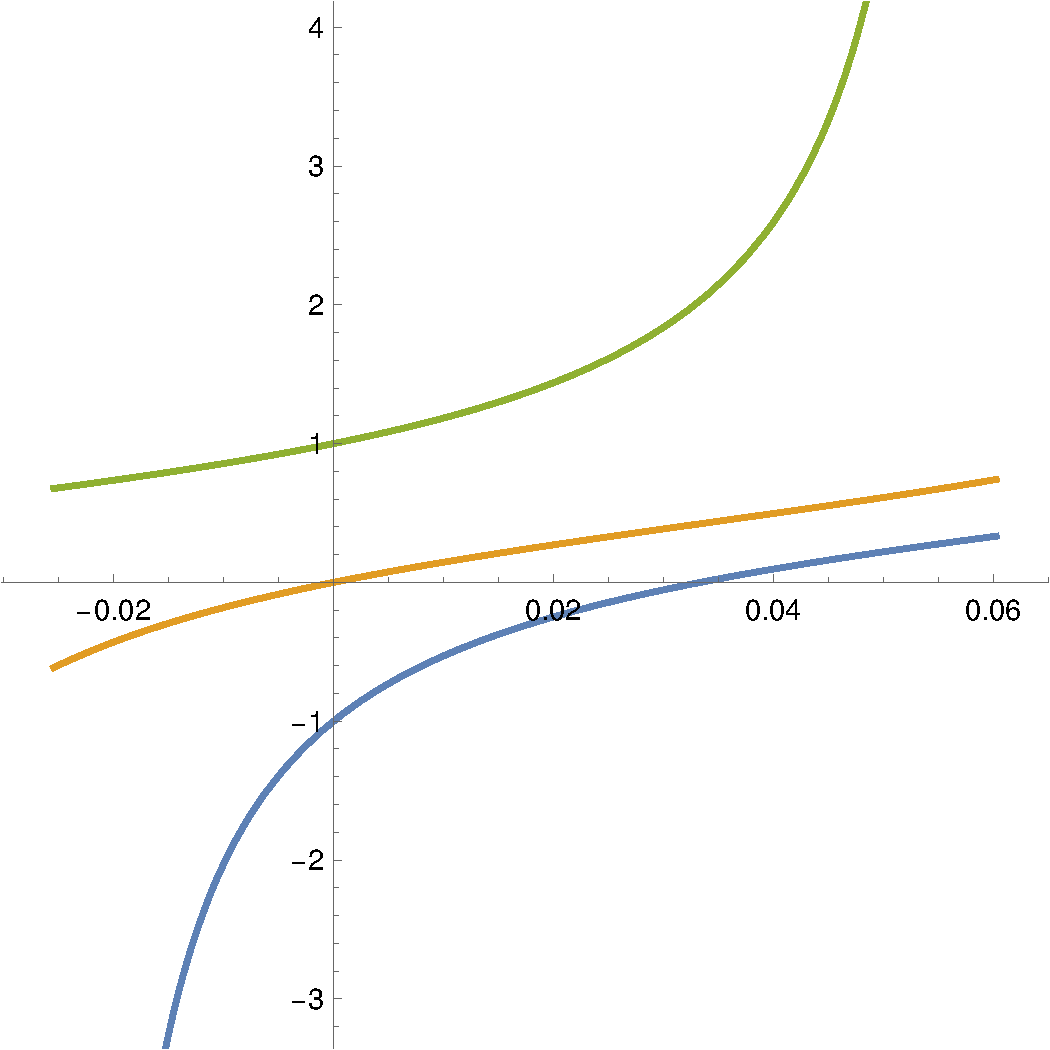
\includegraphics[width=\textwidth]{graphs/3N/x.pdf}
        \caption{First graph}
    \end{subfigure}
	\hfill
	\begin{subfigure}{0.44\textwidth}
		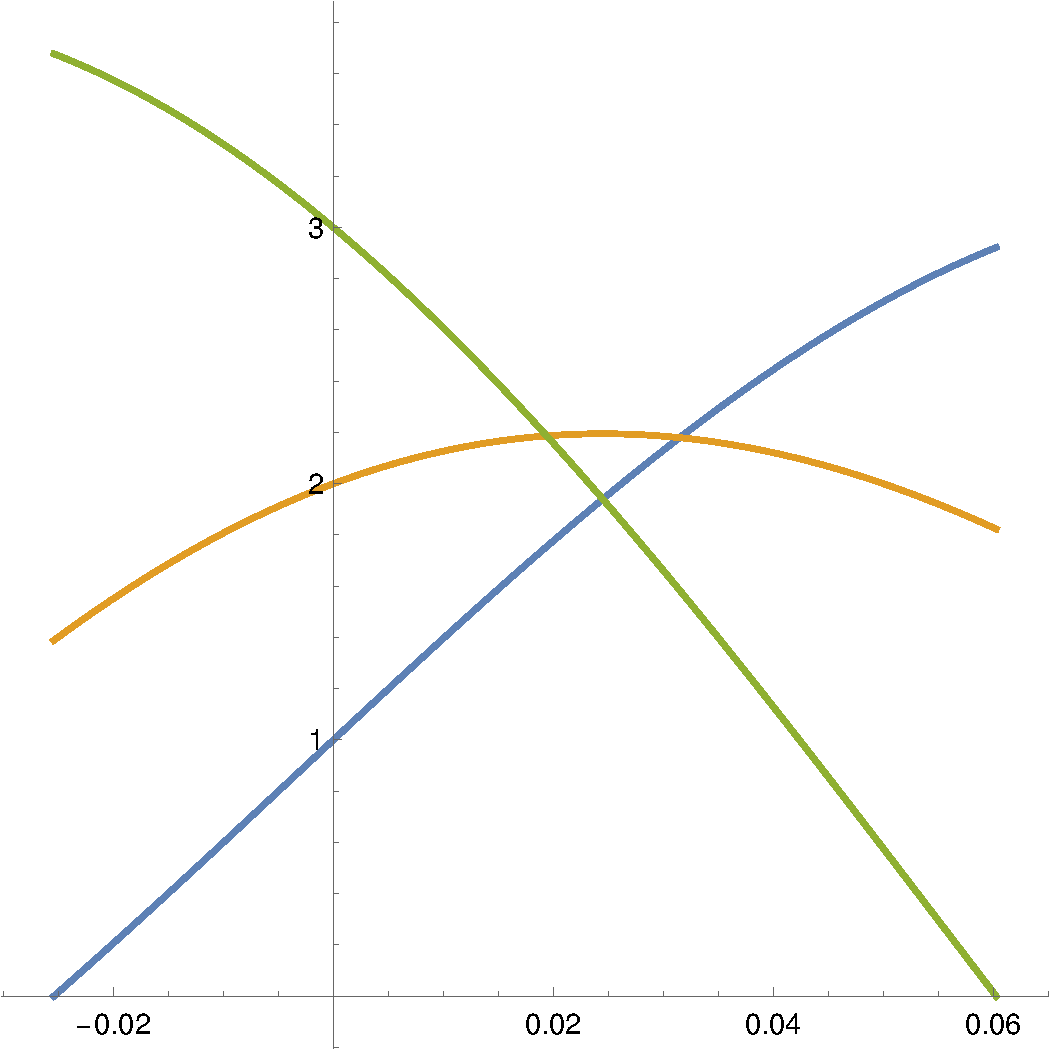
\includegraphics[width=\textwidth]{graphs/3N/m.pdf}
        \caption{First graph2}
    \end{subfigure}
    \caption{$m_1 = 1$, $x_1 = 0$, $m_1 = 2$, $x_2 = 3$}
\end{figure}
It follows the same pattern as the $N = 2$ case were it quickly diverges to infinity.

If $m_k < 0$ and $N > 2$ we have that the peakons can collide. This can be seen in the following graph
\begin{figure}[H]
	\begin{subfigure}{0.44\textwidth}
		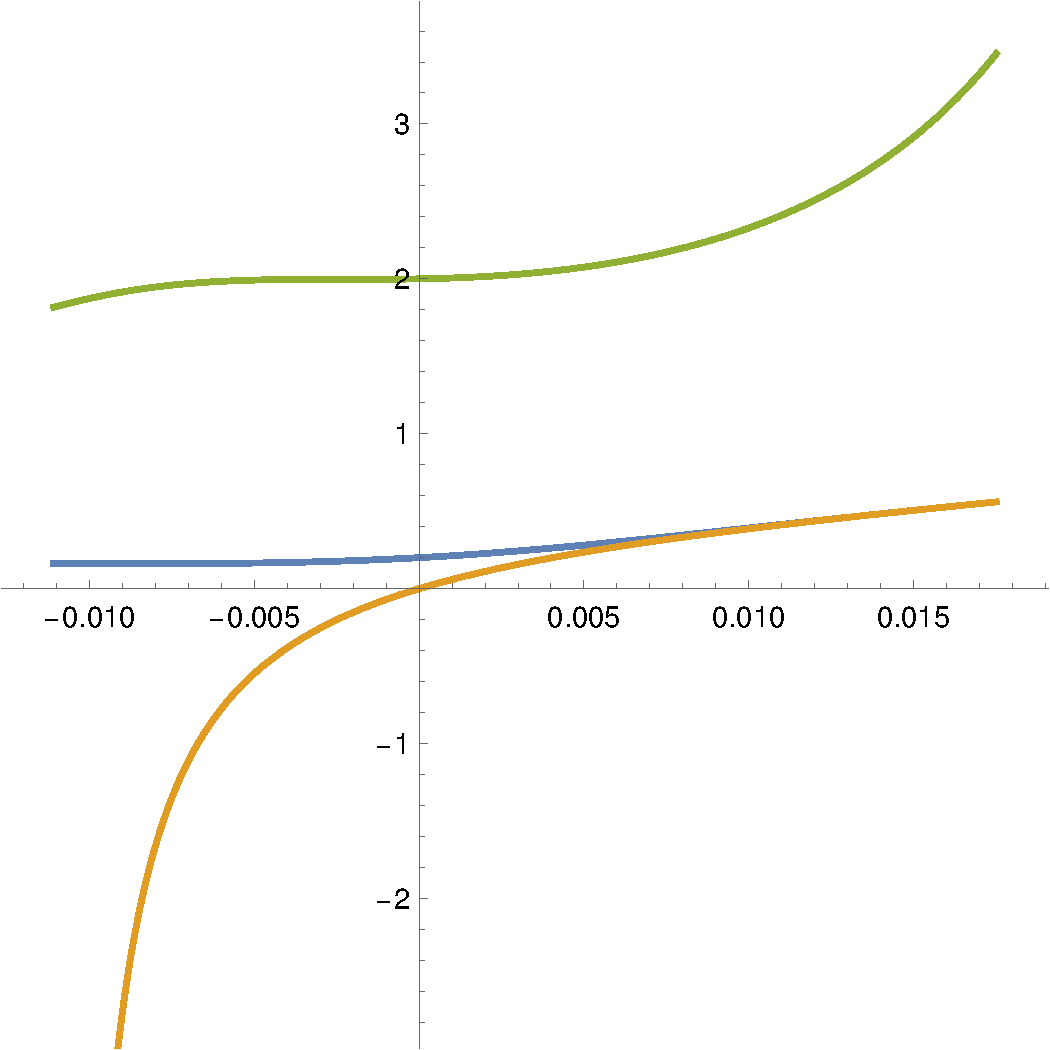
\includegraphics[width=\textwidth]{graphs/3NCollision/x.pdf}
        \caption{First graph}
    \end{subfigure}
	\hfill
	\begin{subfigure}{0.44\textwidth}
		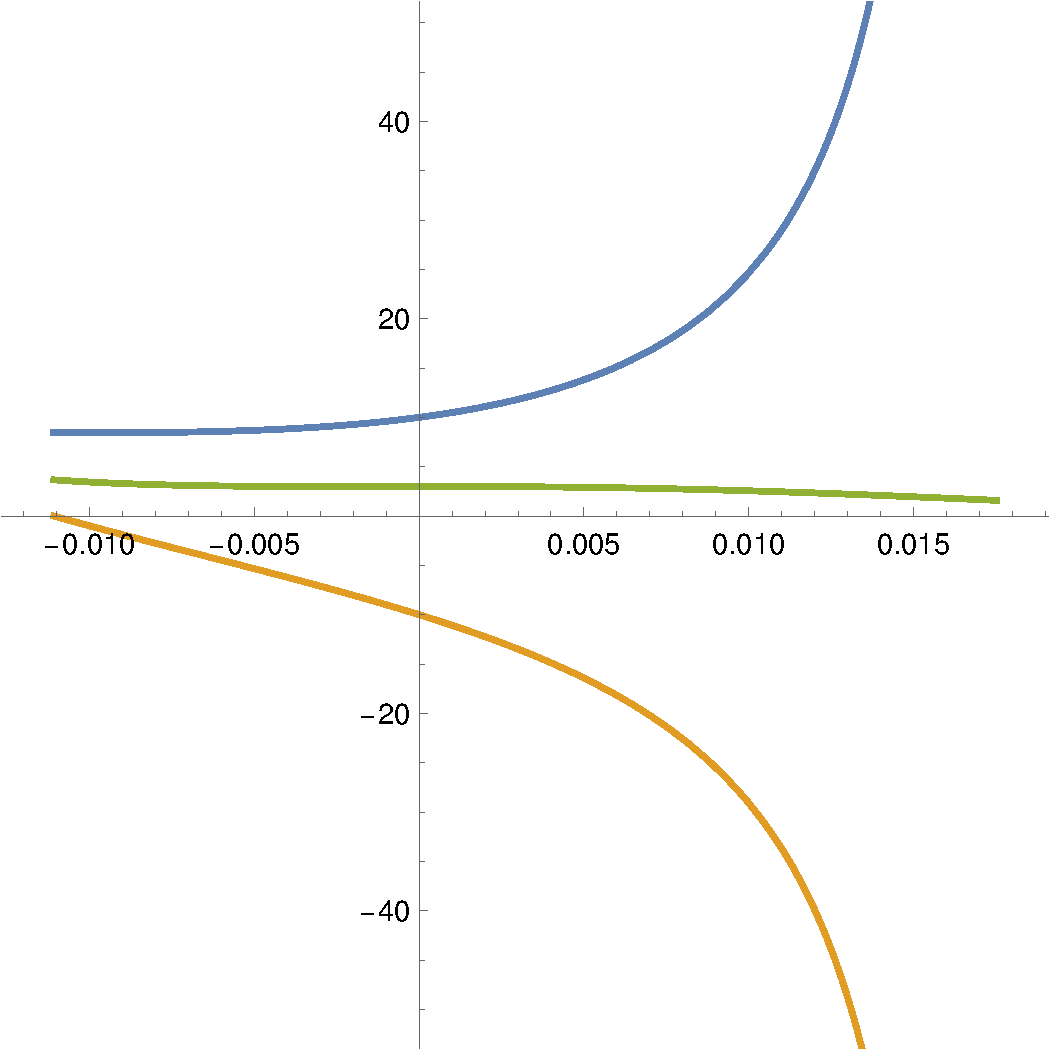
\includegraphics[width=\textwidth]{graphs/3NCollision/m.pdf}
        \caption{First graph}
    \end{subfigure}
    \caption{$m_1 = 1$, $x_1 = 0$, $m_1 = 2$, $x_2 = 3$}
\end{figure}

Next, we will take a look at the case where we continue the solution after the peakons have diverged to infinity.
\begin{figure}[H]
	\begin{subfigure}{0.44\textwidth}
		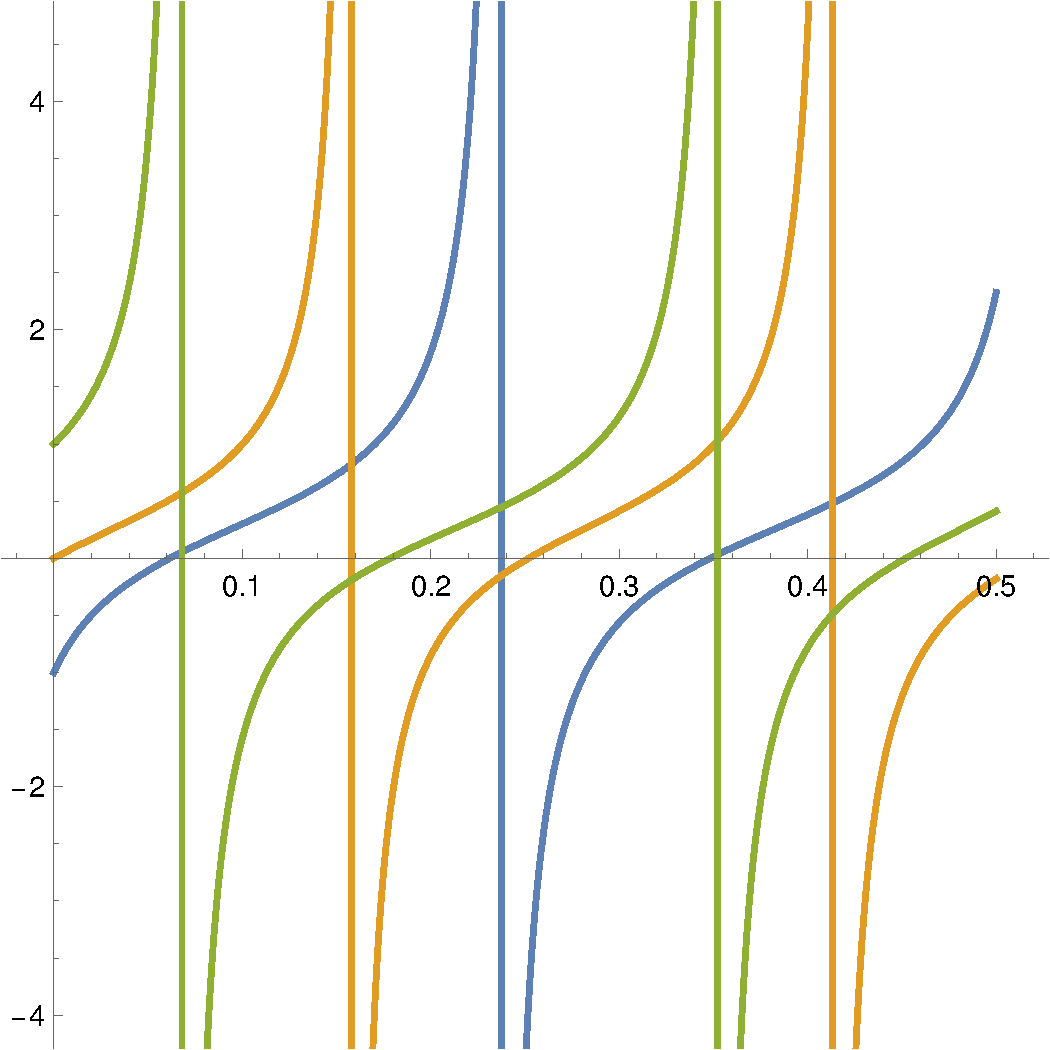
\includegraphics[width=\textwidth]{graphs/3NInfinite/x.pdf}
        \caption{First graph}
    \end{subfigure}
	\hfill
	\begin{subfigure}{0.44\textwidth}
		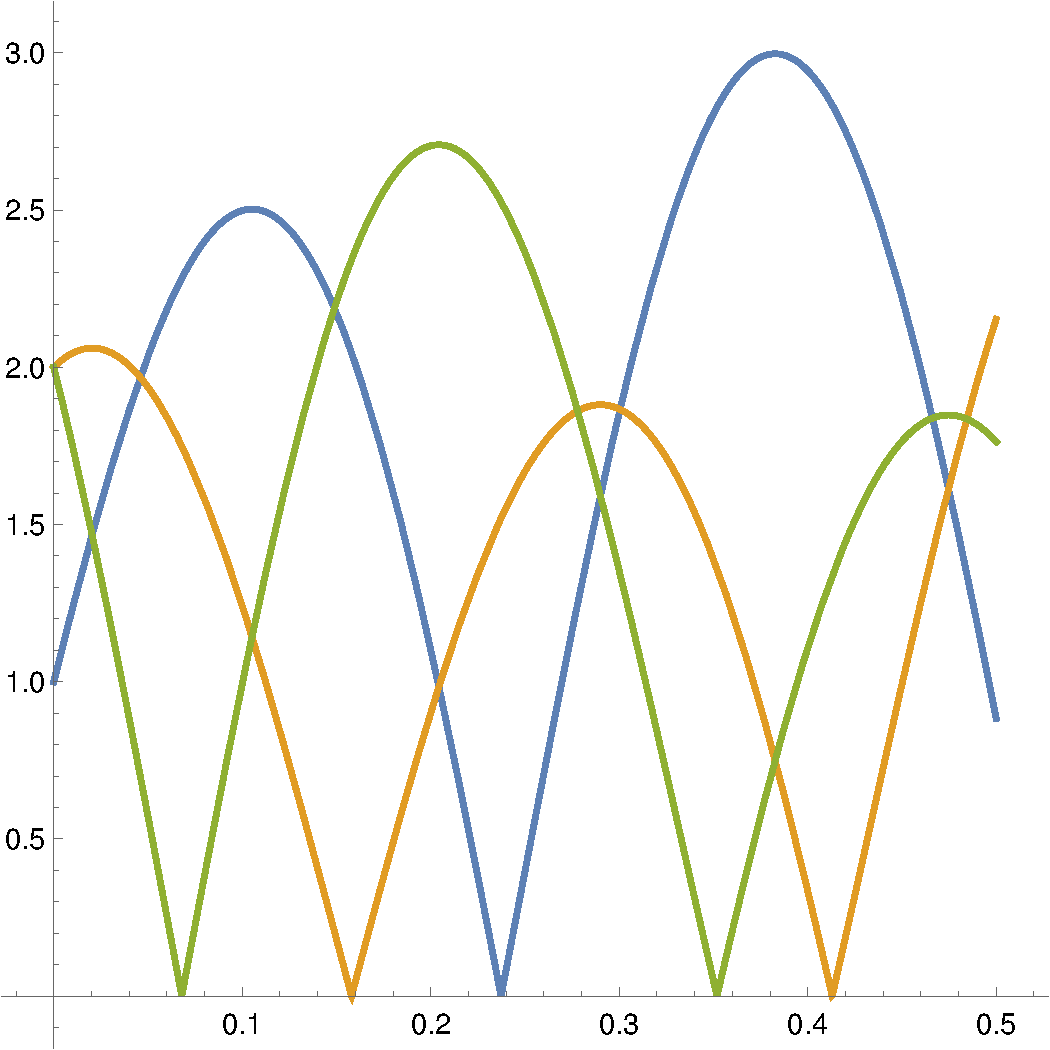
\includegraphics[width=\textwidth]{graphs/3NInfinite/m.pdf}
        \caption{First graph}
    \end{subfigure}
    \caption{$m_1 = 1$, $x_1 = 0$, $m_1 = 2$, $x_2 = 3$}
	\label{fig:3N}
\end{figure}
Here, in figure (\ref{fig:3N}), it can be observed that the $x_i$ and $m_i$ behaves very closely to the $N = 2$ case. The $x_i$ is still the same shape as $\tan(t)$ and $m_i$ is still the same shape as $|\sin(t)|$.

\begin{figure}[H]
	\begin{subfigure}{0.44\textwidth}
		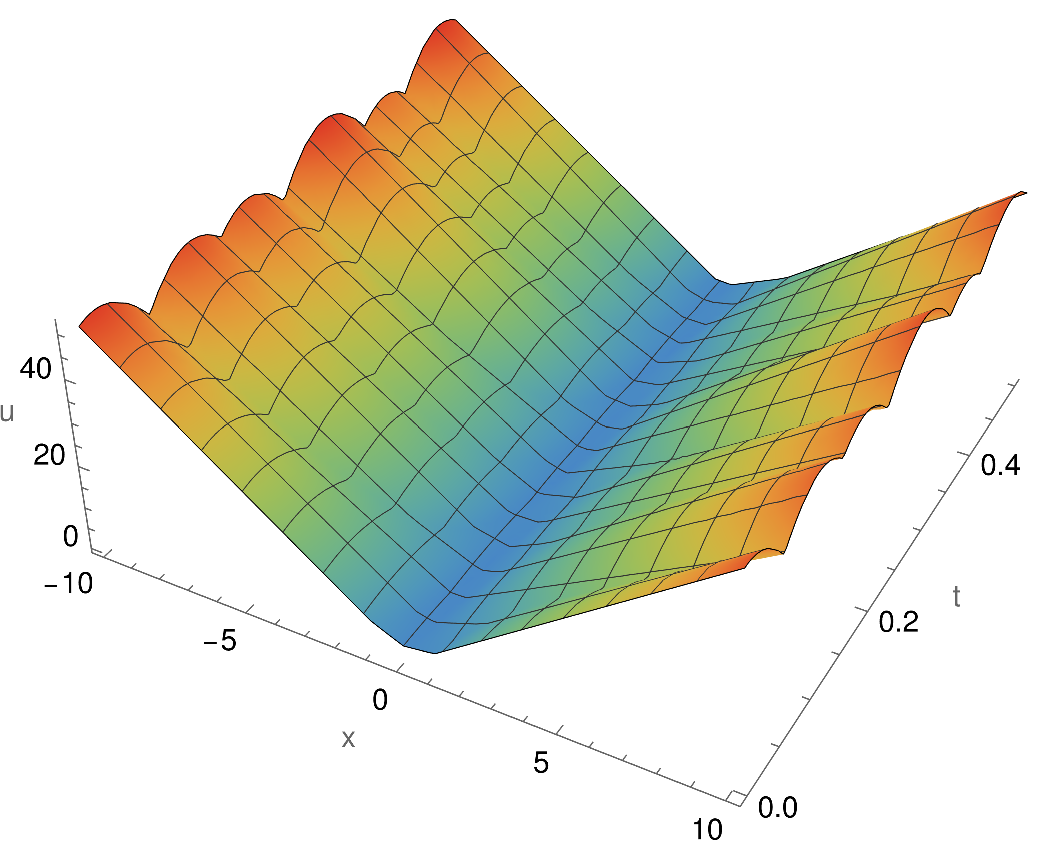
\includegraphics[width=\textwidth]{graphs/3NInfinite/u3D.pdf}
        \caption{First graph}
    \end{subfigure}
	\hfill
	\begin{subfigure}{0.44\textwidth}
		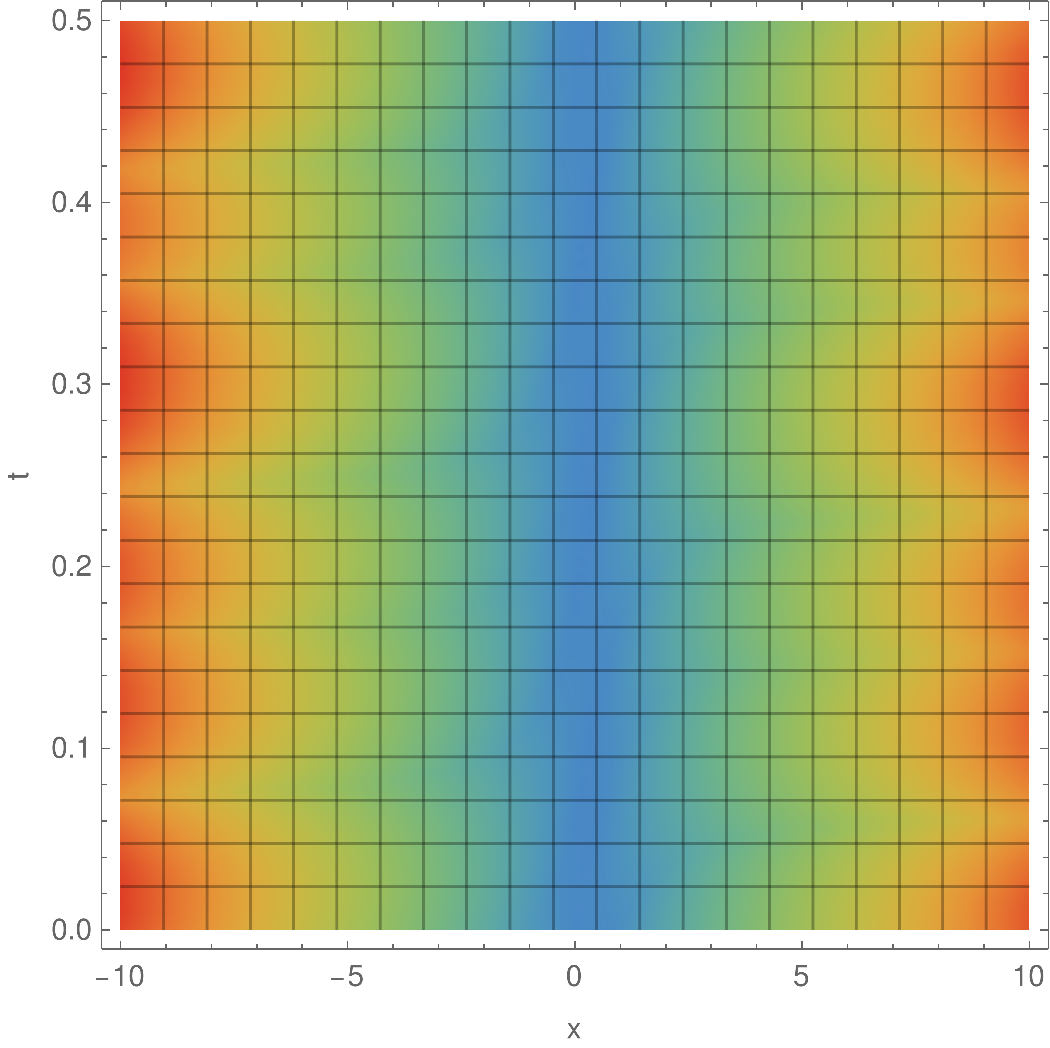
\includegraphics[width=\textwidth]{graphs/3NInfinite/u2D.pdf}
        \caption{First graph}
    \end{subfigure}
    \caption{$m_1 = 1$, $x_1 = 0$, $m_1 = 2$, $x_2 = 3$}
	\label{fig:u3N}
\end{figure}
In figure (\ref{fig:u3N}) it can be observed the function behaves like the absolute function with increasing fluctuations away from a center position. The fluctuations scale linearly with the distance from the center. The behavior of $u(x, t)$ for $x$ far from the center is
\begin{equation}
	\lim_{x \to \infty} u(x, t) = \lim_{x \to \infty} \sum_{k = 1}^{N} m_k |x - x_k| = \sum_{k = 1}^{N} m_k |x| + \sgn(x)x_k
\end{equation}
What is interesting here is that the center seems to not be moving from it's inital position.
\begin{figure}[H]
	\begin{subfigure}{0.44\textwidth}
		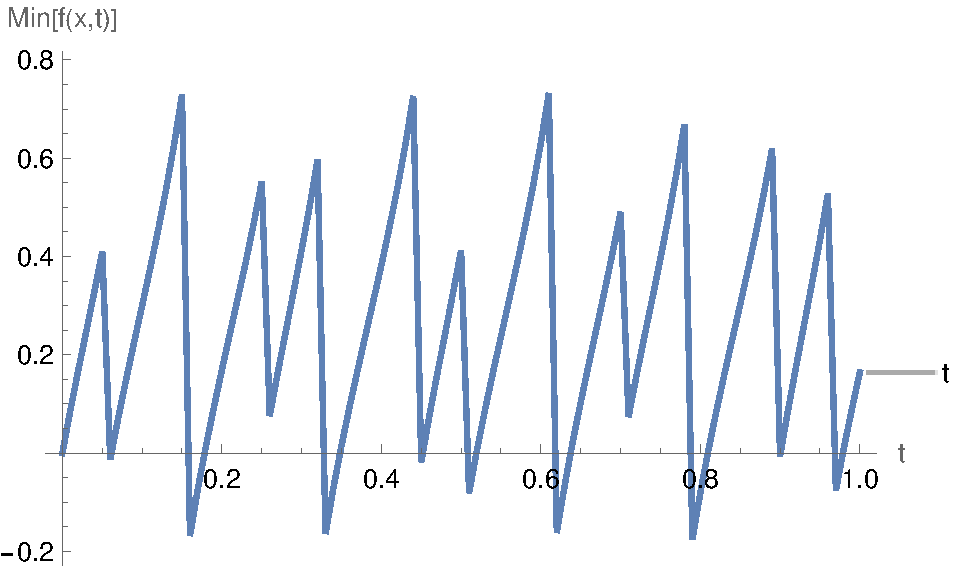
\includegraphics[width=\textwidth]{graphs/3NInfinite/uMin.pdf}
        \caption{First graph}
    \end{subfigure}
	\hfill
	\begin{subfigure}{0.44\textwidth}
		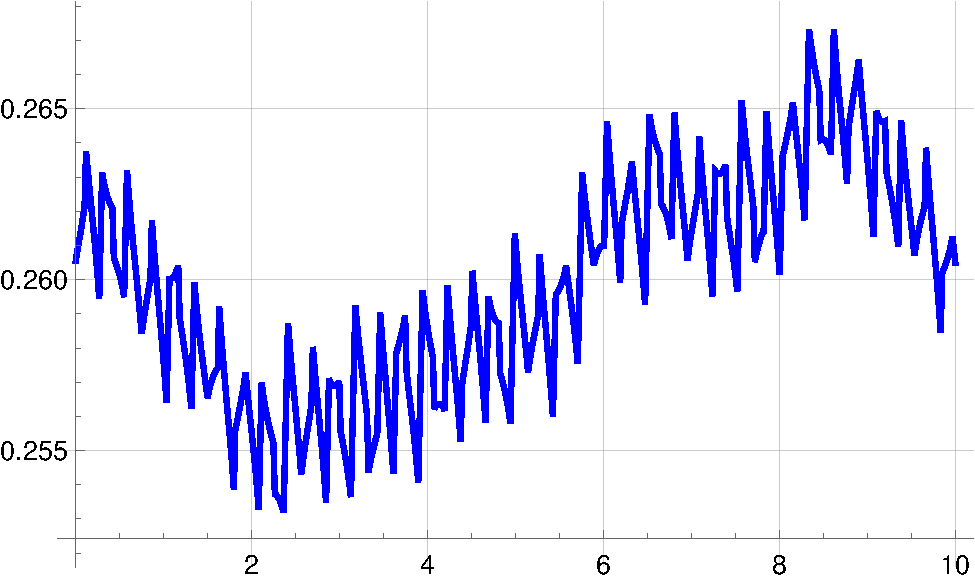
\includegraphics[width=\textwidth]{graphs/3NInfinite/movingAvg.pdf}
        \caption{First graph}
    \end{subfigure}
    \caption{$m_1 = 1$, $x_1 = 0$, $m_1 = 2$, $x_2 = 3$}
\end{figure}
Even though the minimum of the function $u(x, t)$ varies it fluctuates around a constant value as can be seen in figure (\ref{fig:uCenter}).

\subsection{Periodic HF Novikov equation}

For the periodic graphs the boundary conditions are that $u(x,t)$ is periodic with period $L$. $L$ is set to $10$ for all simulations.

First we will look at the graph of the function $u(x, t)$.
\begin{figure}[H]
	\begin{subfigure}{0.44\textwidth}
		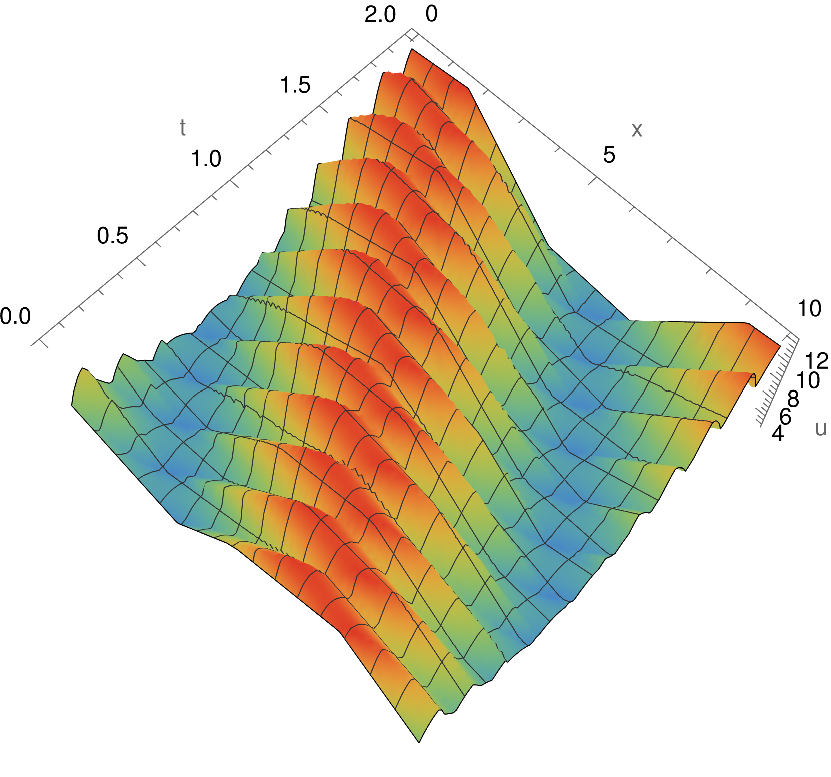
\includegraphics[width=\textwidth]{graphs/per2N/u3D.pdf}
        \caption{First graph}
    \end{subfigure}
	\hfill
	\begin{subfigure}{0.44\textwidth}
		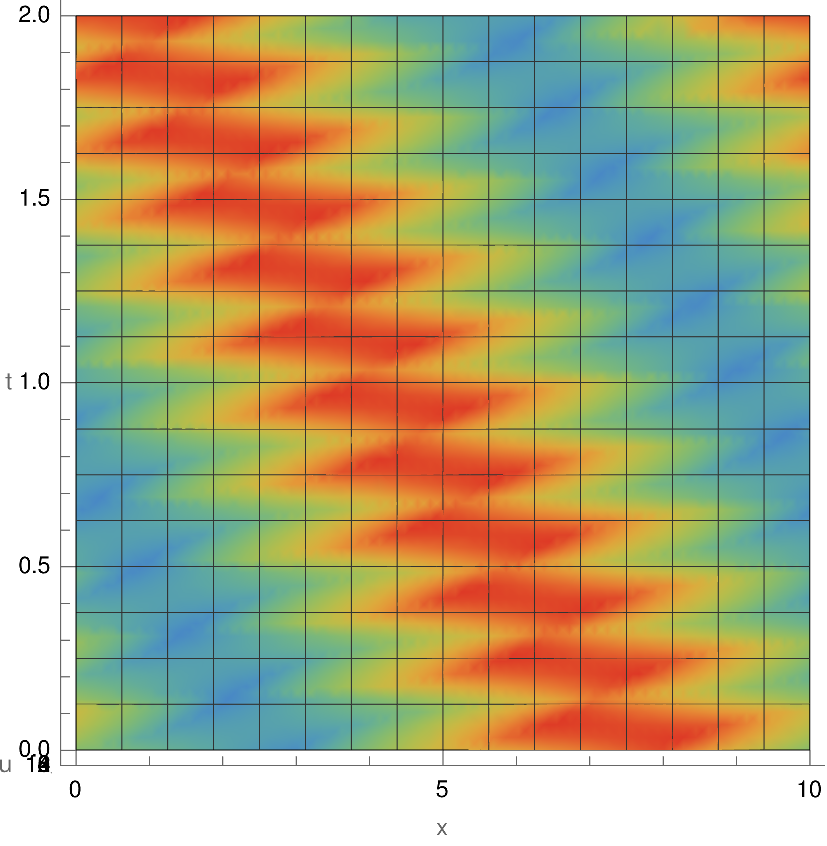
\includegraphics[width=\textwidth]{graphs/per2N/u2D.pdf}
        \caption{First graph}
    \end{subfigure}
    \caption{$m_1 = 1$, $x_1 = 0$, $m_1 = 2$, $x_2 = 3$}
    \label{fig:u2N}
\end{figure}
In figure (\ref{fig:u2N}) it can be observed the function behaves like a wave of constant speed with internal fluctuations. This have been observed for all $N$ and all initial conditions where $m_k > 0$.
\begin{figure}[H]
	\begin{subfigure}{0.44\textwidth}
		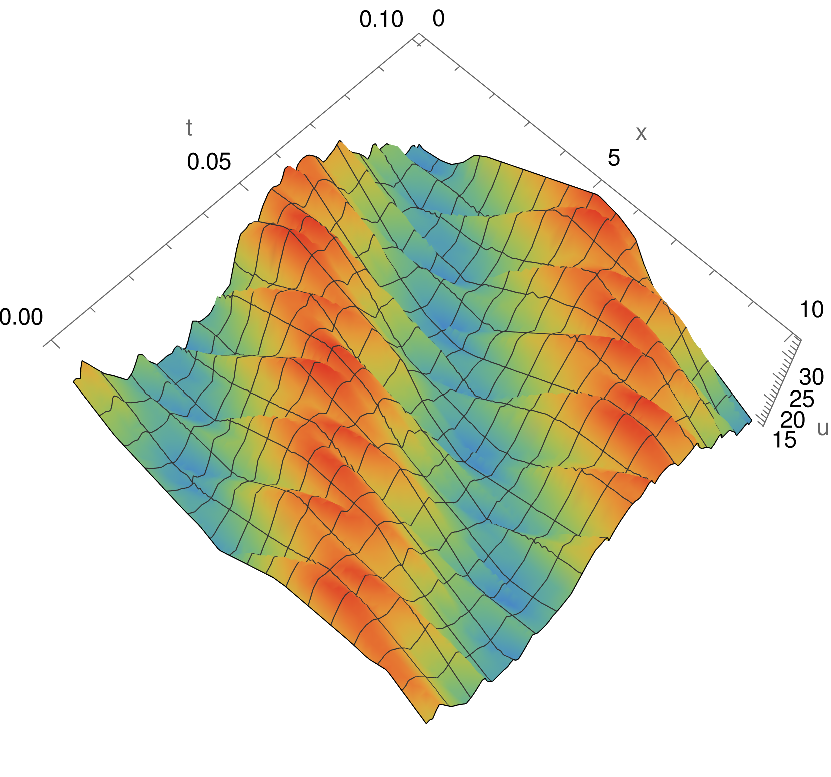
\includegraphics[width=\textwidth]{graphs/per4N/u3D.pdf}
        \caption{First graph}
    \end{subfigure}
	\hfill
	\begin{subfigure}{0.44\textwidth}
		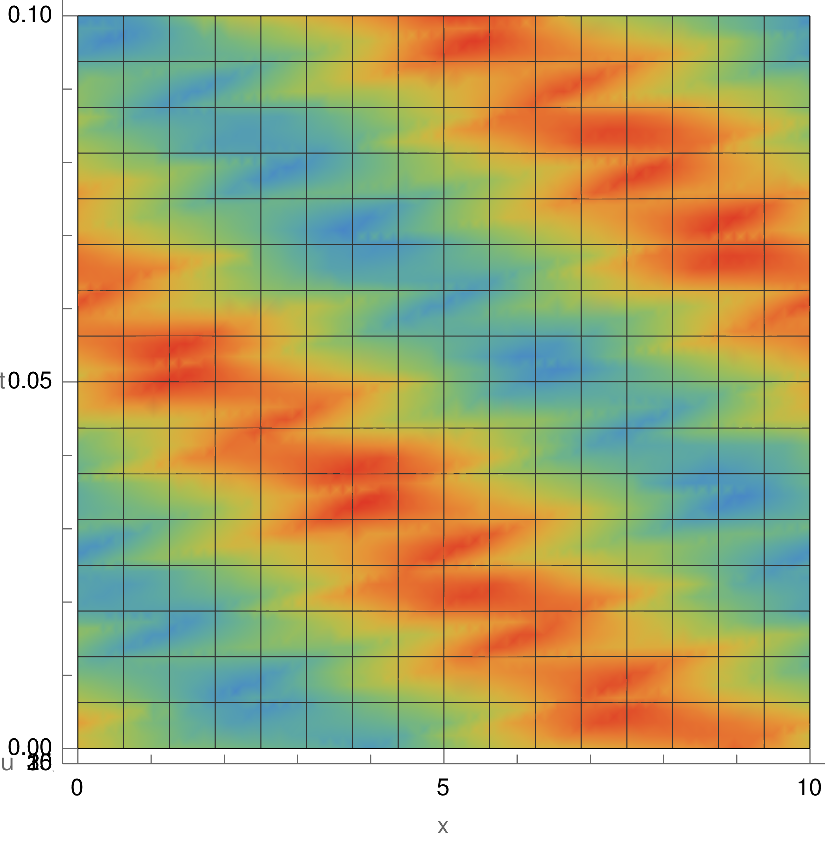
\includegraphics[width=\textwidth]{graphs/per4N/u2D.pdf}
        \caption{First graph}
    \end{subfigure}
    \caption{$m_1 = 2, x_1 = 1, m_1 = 0.5, x_2 = 3, m_3 = 5, x_3 = 4, m_4 = 2, x_4 = 8.5$}
\end{figure}

\begin{figure}[H]
	\begin{subfigure}{0.3\textwidth}
        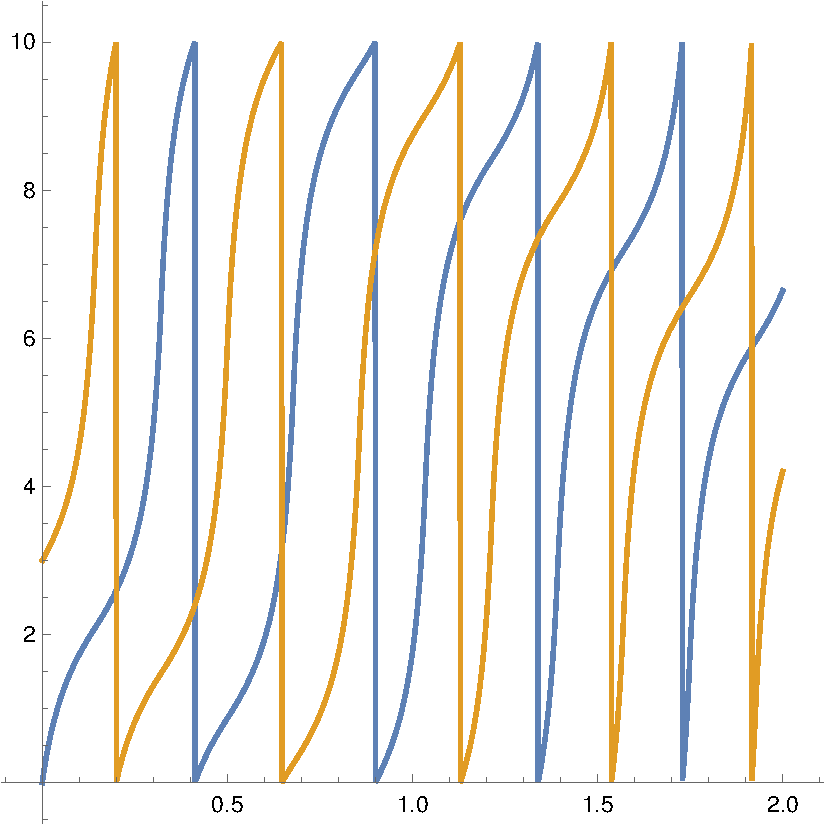
\includegraphics[width=\textwidth]{graphs/per2N/x.pdf}
        \caption{First graph}
    \end{subfigure}
	\hfill
	\begin{subfigure}{0.3\textwidth}
        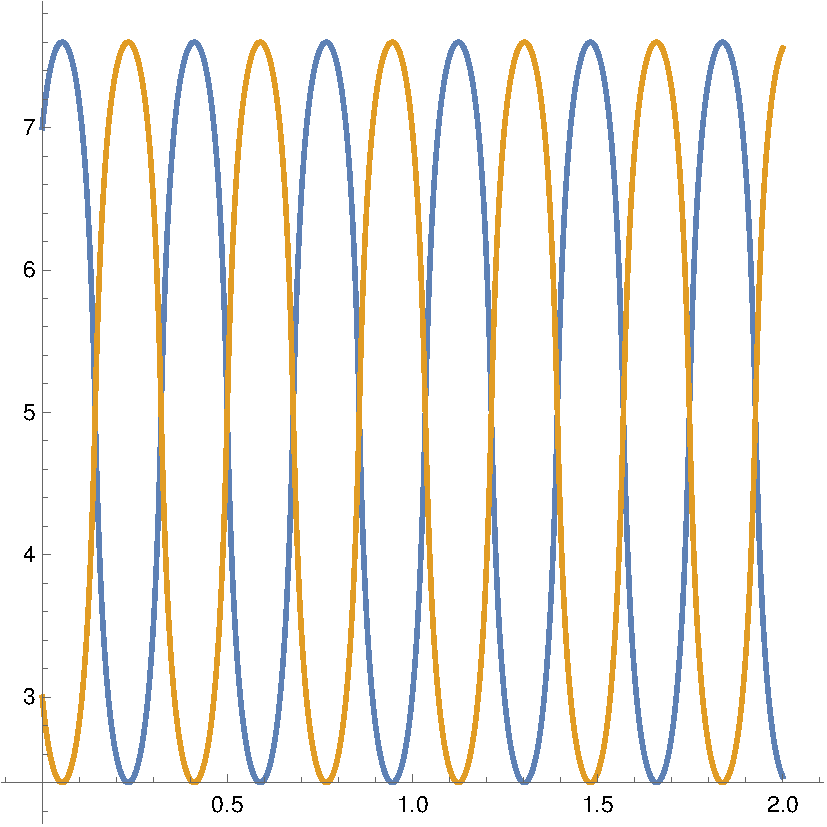
\includegraphics[width=\textwidth]{graphs/per2N/xDist.pdf}
        \caption{First graph}
    \end{subfigure}
	\hfill
	\begin{subfigure}{0.3\textwidth}
        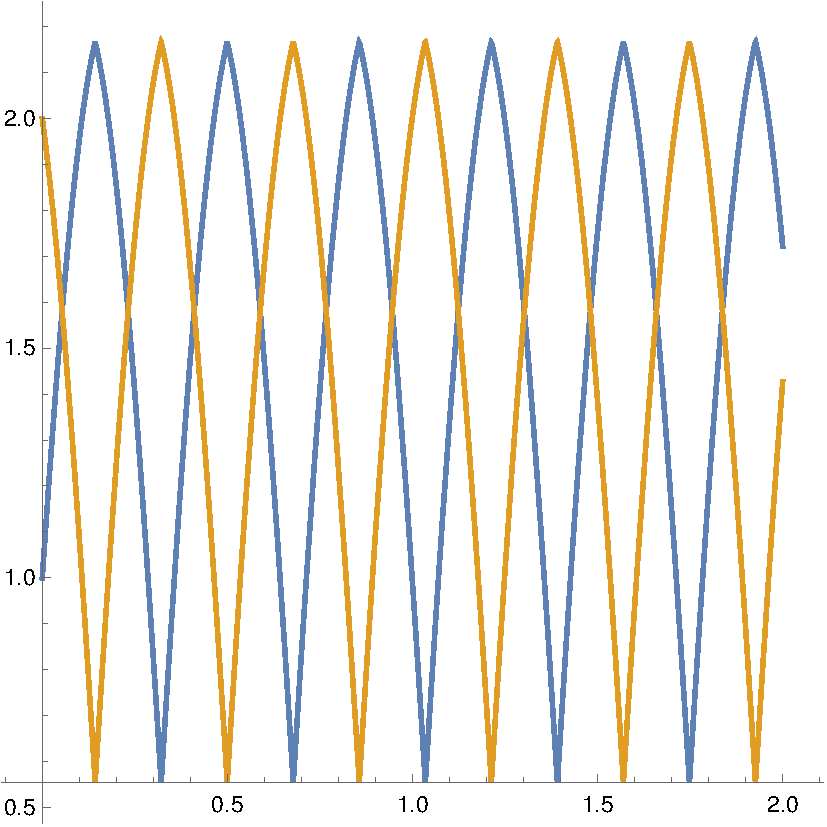
\includegraphics[width=\textwidth]{graphs/per2N/m.pdf}
        \caption{First graph}
    \end{subfigure}
    \caption{$m_1 = 2, x_1 = 1, m_1 = 0.5, x_2 = 3, m_3 = 5, x_3 = 4, m_4 = 2, x_4 = 8.5$}
\end{figure}

\begin{figure}[H]
	\begin{subfigure}{0.3\textwidth}
        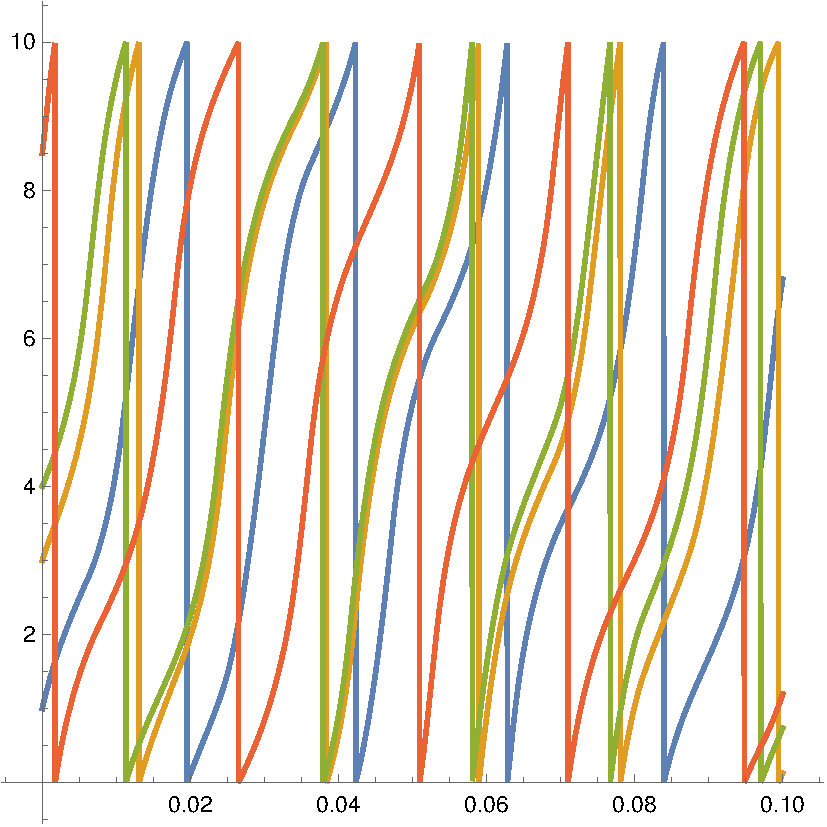
\includegraphics[width=\textwidth]{graphs/per4N/x.pdf}
        \caption{First graph}
    \end{subfigure}
	\hfill
	\begin{subfigure}{0.3\textwidth}
        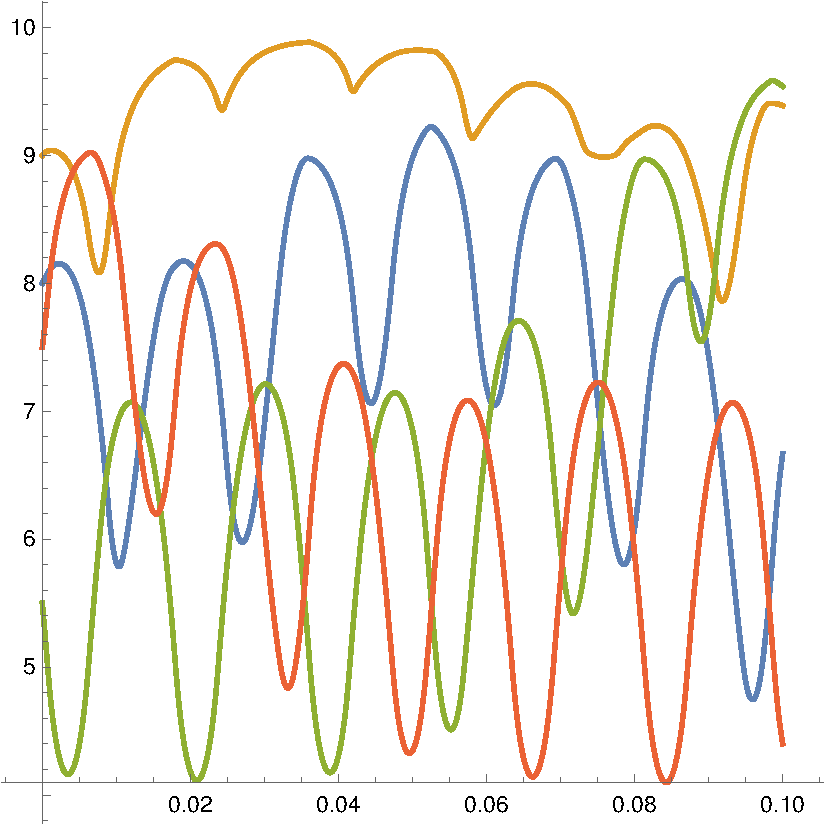
\includegraphics[width=\textwidth]{graphs/per4N/xDist.pdf}
        \caption{First graph}
    \end{subfigure}
	\hfill
	\begin{subfigure}{0.3\textwidth}
        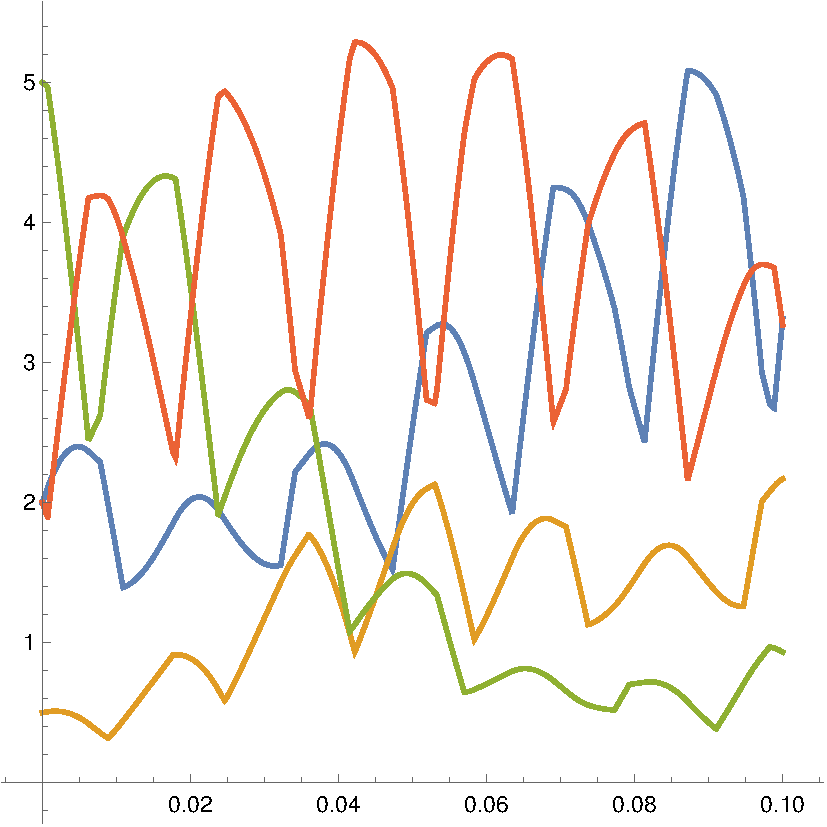
\includegraphics[width=\textwidth]{graphs/per4N/m.pdf}
        \caption{First graph}
    \end{subfigure}
    \caption{$m_1 = 2, x_1 = 1, m_1 = 0.5, x_2 = 3, m_3 = 5, x_3 = 4, m_4 = 2, x_4 = 8.5$}
\end{figure}

Just as for the non periodic case when $m_k < 0$ and $N > 2$ the peakons can collide.
\begin{figure}[H]
	\begin{subfigure}{0.3\textwidth}
        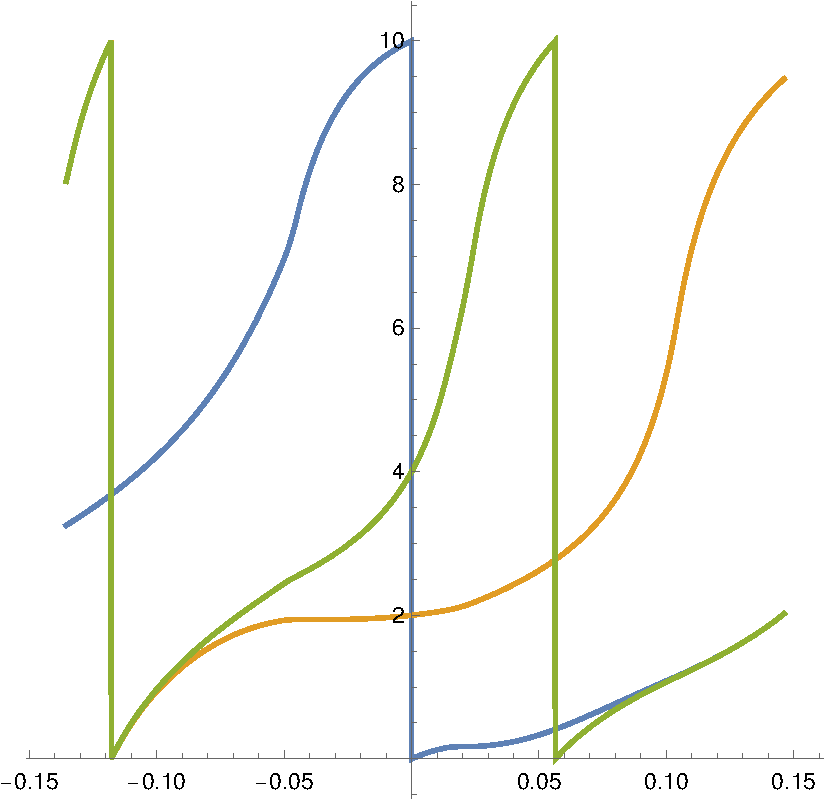
\includegraphics[width=\textwidth]{graphs/perCollision/x.pdf}
        \caption{First graph}
    \end{subfigure}
	\hfill
	\begin{subfigure}{0.3\textwidth}
        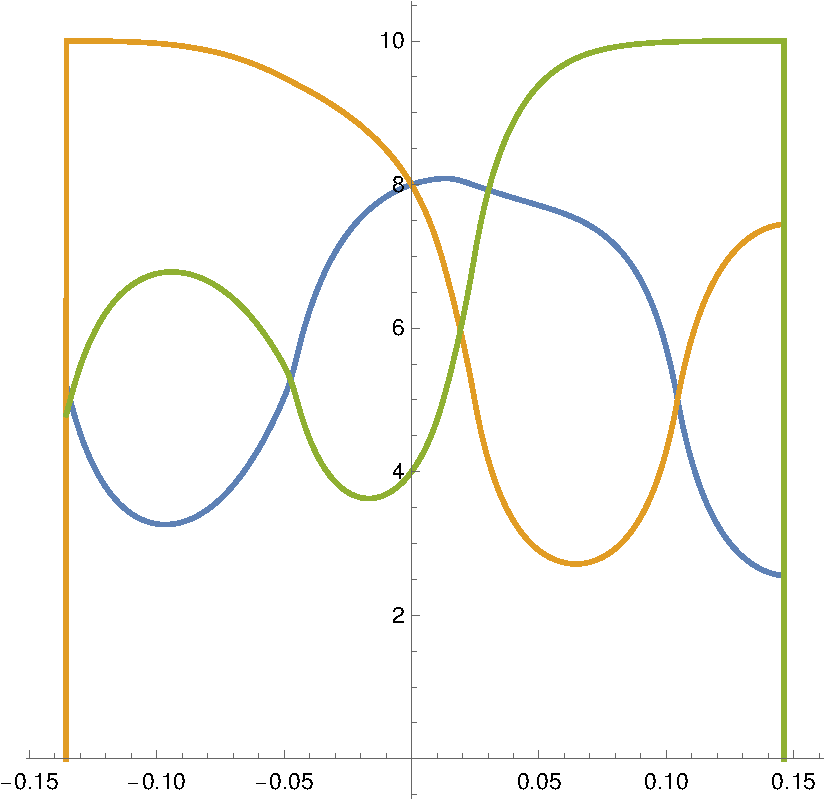
\includegraphics[width=\textwidth]{graphs/perCollision/xDist.pdf}
        \caption{First graph}
    \end{subfigure}
	\hfill
	\begin{subfigure}{0.3\textwidth}
        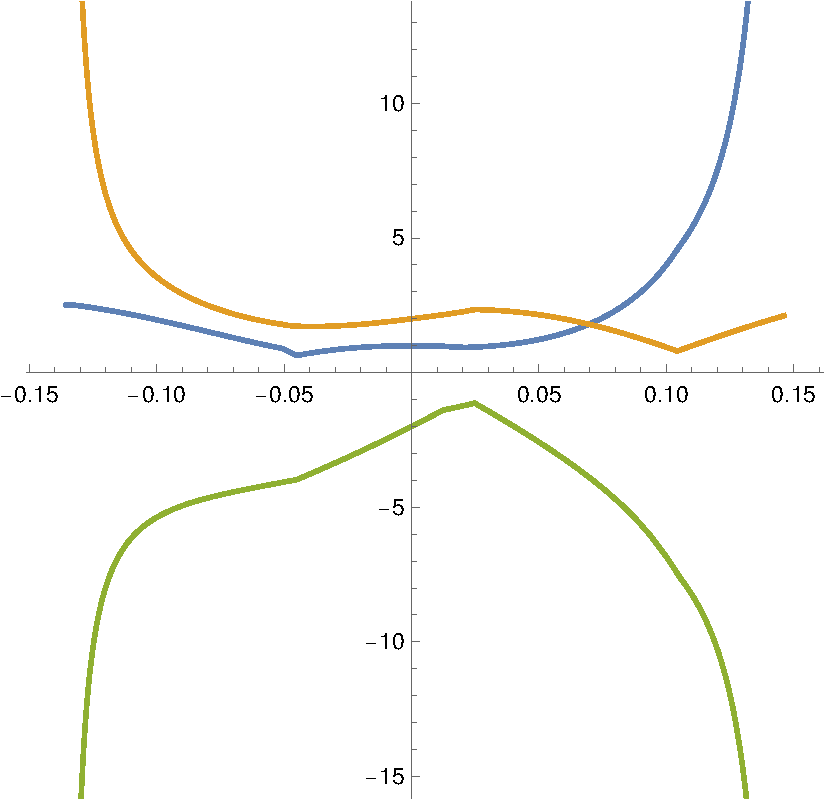
\includegraphics[width=\textwidth]{graphs/perCollision/m.pdf}
        \caption{First graph}
    \end{subfigure}
    \caption{$m_1 = 2, x_1 = 1, m_1 = 0.5, x_2 = 3, m_3 = 5, x_3 = 4, m_4 = 2, x_4 = 8.5$}
\end{figure}


% 55:00
\section{Hamiltonian structure}

% We tried to find a Hamiltonian structure for the HF Novikov equation. 

\todo{Todo: Add references}

The Hamiltonian formalism is a fundamental framework that offers a powerful method for analyzing dynamical systems. The state of the system is described by a set of canonical coordinates
\begin{equation}
	 (q_i,p_i), \qquad i = 1,\dots,n.
\end{equation}
In the context of peakon ODEs, the canonical coordinates are the peakon positions $x_i$ and the peakon momenta $m_i$. The Hamiltonian $H(q,p,t)$ is a function representing the total energy or another conserved quantity of the system. It is expressed in terms of the canonical coordinates and possibly time. The evolution of the system is governed by Hamilton's equations, which take the form
%
\begin{equation}
\begin{pmatrix}
	\dot{q} \\
	\dot{p}
\end{pmatrix} =
\Pi(x)
\begin{pmatrix}
	\partial H / \partial q \\
	\partial H / \partial p
\end{pmatrix}.
\end{equation}
%
Or as
%
\begin{equation}
	\dot{x} = \Pi(x) \nabla H(x),
\end{equation}
%
where $x = (q,p)$, $\nabla H(x) = (\partial H / \partial q, \partial H / \partial p)$. 
The Poisson matrix has to be skew-symmetric, $\Pi^T = -\Pi$, and satisfy the Jacobi identity
\begin{equation}
	\{\{f,g\},h\} + \{\{g,h\},f\} + \{\{h,f\},g\} = 0.
\end{equation}
%
where the Poisson brackets is defined as
%
\begin{equation}
	\{f,g\} = (\nabla f)^T \Pi \nabla g.	
\end{equation}
%
For the canonical coordinates it's defined as
%
\begin{align}
	\{x_i, x_j\} &= \Pi^{ij}(x), \\
	\{\{x_i, x_j\}, x_k\} &= \sum_{l=1}^n \Pi^{lk}(x) \frac{\partial}{\partial x_l} \Pi^{ij}(x).
\end{align}
%
A common way to construct the Hamiltonian structure is to use the canonical Poisson matrix
%
\begin{equation}
\begin{pmatrix}
	\dot{q} \\
	\dot{p}
\end{pmatrix} =
\begin{pmatrix}
	0 & I \\
	-I & 0
\end{pmatrix}
\begin{pmatrix}
	\partial H / \partial q \\
	\partial H / \partial p
\end{pmatrix},
\end{equation}
%
or as
%
\begin{equation}
	\dot{q}_i = \frac{\partial H}{\partial p_i}, \quad
	\dot{p}_i = -\frac{\partial H}{\partial q_i}.
\end{equation}
%
where I is the $n \times n$ identity matrix. A more general form of the Hamiltonian structure is with the $2n \times 2n$ Poisson matrix $\Pi$, where the equations of motion are instead written as

A finite dimensional Hamiltonian system is integrable if it possesses as many conserved quantities $F_i$ as degrees of freedom, and these quantities are in involution
%
\begin{equation}
	\{F_i, F_j\} = 0.
\end{equation}
%
These conserved quantities allow the system's equations of motion to in principle be solved explicitly. 

\subsection{Comparison to other soliton equations}

Here we will show the Hamiltonian structure for the CH, DP, and Novikov peakon ODEs as well as the Hunter Saxton peakon ODE, which is the only HF peakon ODE that has a known Hamiltonian structure. The non HF peakon ODEs Hamiltonian structure can be written on the common form
\begin{alignat}{3}
	\{&x_i, &x_j\} &= \phantom{-}G(x_i - x_j), \\
	\{&x_i, &m_j\} &= \phantom{-}G'(x_i - x_j)m_j (b - 1), \\
	\{&m_i, &m_j\} &=           -G''(x_i - x_j) m_i m_j (b - 1)^2,
	G(x) = A \sgn(x) (1 - e^{-B|x|}),
\end{alignat}
%
with the paramters and Hamilton function given in the table below:
\begin{center}
  \begin{tabular}{l|c|c|c|c}
    & $A$ & $B$ & $b$ & $H$ \\
    \hline
    Camassa--Holm
	& $1$ & $1$ & $2$ & $\sum m_i$ \\
    \hline
    Degasperis--Procesi
	& $1/2$ & $1$ & $3$ & $\sum m_i$ \\
    \hline
    Novikov
	& $1$ & $2$ & $3/2$ & $\sum m_i m_j e^{-|x_i - x_j|}$ \\
  \end{tabular}
\end{center}
%
The Hunter Saxton's Hamiltonian structure is given by the canonical Poisson matrix
\begin{equation}
	\{m_i, x_i\} = \delta_{ij} \quad \{m_i, m_j\} = 0 = \{x_i, x_j\}
\end{equation}
and the Hamiltonian
\begin{equation}
	H = \frac{1}{2} \sum m_i m_j |x_i - x_j|,
\end{equation}
which can be related to another similar Hamiltonian structure of Camassa--Holm that also has the canonical Poisson matrix but with the Hamiltonian 
\begin{equation}
	H = \frac{1}{2} \sum m_i m_j e^{-|x_i - x_j|}.
\end{equation}
%
We wanted to find a Hamiltonian structure for the HF Novikov peakon ODEs but it was harder than expected. The search for a Hamiltonian structure was done by trying to start from the Novikov Hamiltonian structure and try to modify it to fit the HF Novikov peakon ODEs. If the search is continued in the future, a more structured approach should be taken. Finding a Hamiltonian for the Novikov PDE could be a good starting point and has been the method used to find the other Hamiltonians for the peakon ODEs.

\section{Constants of motion by direct search}

Two methods have been used to find constants of motion for the HF Novikov equation. One of the methods will be covered in the next section. The other method is an exhaustive search algorithm. The algorithm is based on the assumption that the constants of motion are polynomials in the variables $m_k$ and $x_k$ of a fixed degree $M$ and $X$ for $m_k$ respectively $x_k$. The algorithm lists all monomials of that fixed degree
\begin{equation}
	\prod_{i=1}^{N} m_i^{a_i} x_i^{b_i},
\end{equation}
where the sum of $a_i$ is $M$ and the sum of $b_i$ is $X$. The algorithm then takes the time derivative of each monomial and forms a linear combination of them. The constants of motion are then found by finding linear combinations that are zero. The algorithm has been run both symbolically in Mathematica and numerically in C++. The algorithm has been successful up until $N = 4$, where time and numerical precision become limiting factors.

\subsection*{Jacobian method}
Two or more constants of motion are said to be functionally independent if none of them can be expressed as a function of the others. In other words, they provide unique information about the system.

To determine if a set of constants of motion are independent, the Jacobian matrix is used. Suppose there are a set of $n$ constants of motion $M_1,M_2,\dots,M_m$. These constants are functions of the variables $x_1,x_2,\dots,x_n,m_1,m_2,\dots,m_n$.

The Jacobian matrix $J$ of the functions ${M_1,M_2,\dots,M_m}$ with respect to the variables ${x_1,x_2,\dots,x_n,m_1,m_2,\dots,m_n}$ is given by:

\begin{equation}
	j = 
	\begin{pmatrix}
		\frac{\partial m_1}{\partial x_1} & \frac{\partial m_1}{\partial x_2} & \cdots & \frac{\partial m_1}{\partial x_n} & \frac{\partial m_1}{\partial m_1} & \frac{\partial m_1}{\partial m_2} & \cdots & \frac{\partial m_1}{\partial m_n} \\
		\frac{\partial m_2}{\partial x_1} & \frac{\partial m_2}{\partial x_2} & \cdots & \frac{\partial m_2}{\partial x_n} & \frac{\partial m_2}{\partial m_1} & \frac{\partial m_2}{\partial m_2} & \cdots & \frac{\partial m_2}{\partial m_n} \\
		\vdots & \vdots & \ddots & \vdots & \vdots & \vdots & \ddots & \vdots \\
		\frac{\partial m_n}{\partial x_1} & \frac{\partial m_n}{\partial x_2} & \cdots & \frac{\partial m_n}{\partial x_n} & \frac{\partial m_n}{\partial m_1} & \frac{\partial m_n}{\partial m_2} & \cdots & \frac{\partial m_n}{\partial m_n}
	\end{pmatrix}
\end{equation}

Each row of the Jacobian matrix is the gradient of one of the constants of motion. If the gradients are linearly dependent it means that one of the constants of motion can be expressed as a function of the others. Thus the rank of the Jacobian matrix is the number of independent constants of motion.


\subsection*{N = 2}

The notation for all constants of motion will be $M_{ab}$ where $a$ is the degree of $m_k$ and $b$ is the degree of $x_k$. The algorithm has found the following four conserved quantities for $N = 2$:

\begin{align}
	M_{21A} &= m_1 m_2 (x_2 - x_1), \\
	M_{20\phantom{A}} &= m_1^2\phantom{x_1} + m_2^2\phantom{x_2}, \\
	M_{21B} &= m_1^2 x_1 + m_2^2 x_2, \\
	M_{22\phantom{A}} &= m_1^2 x_1^2 + m_2^2 x_2^2. \\
\end{align}
%
We observe that $M_{20}$ and $M_{21A}$ are equal the constants $M$ and $K$ from the solution of the ODEs (Eqs. \ref{eq:solution_2N_M} \& \ref{eq:solution_2N_K}).
%
The system of ODEs for $N = 2$ only has four variables so the system should have at most three functionally independent constants of motion. It can be seen that
\begin{equation}
	M_{21A}^2 = M_{20}M_{22} - M_{21B}^2.
\end{equation}

\subsection*{N = 3}

The algorithm has found the following five conserved quantities for $N = 3$.  The first two are
\begin{align}
	M_{21} &= m_1m_2(x_2 - x_1) + m_1m_3(x_3 - x_1) + m_2m_3(x_3 - x_2), \\
	M_{63} &= m_1^2m_2^2m_3^2(x_2 - x_1)(x_3 - x_1)(x_3 - x_1).
\end{align}
Let
\begin{align}
	A & = m_1^2(M_{21} + 2m_2m_3(x_3-x_2)), \\
	B & = m_2^2(M_{21} + 2m_1m_3(x_3-x_1)), \\
	C & = m_3^2(M_{21} + 2m_1m_2(x_2-x_1))
\end{align}
then the three other conserved quantities can be written as
\begin{align}
	M_{41} &= A\phantom{x_1} + B\phantom{x_2} + C\phantom{x_3} \\
	M_{42} &= Ax_1 + Bx_2 + Cx_3 \\
	M_{43} &= Ax_1^2 + Bx_2^2 + Cx_3^2
\end{align}
These conserved quantities aren't functionally independent. The Jacobian method shows that there are only four functionally independent conserved quantities. The first constant can be written as
\begin{equation}
	M_{21}^4 = M_{41}M_{43} - M_{42}^2 + 2M_{21}M_{63}.
\end{equation}


\subsection*{N = 4}

For $N = 4$ six conserved quantities have been found. The first two follow the same pattern as for $N = 3$
\begin{align}
	M_{21} = &m_1 m_2 (x_2 - x_1) + m_1 m_3 (x_3 - x_1) + m_1 m_4 (x_4 - x_1) \\ +  &m_2 m_3 (x_3 - x_2) + m_2 m_4 (x_4 - x_2) + m_3 m_4 (x_4 - x_3),\\
	M_{84} = &m_1^2m_2^2m_3^2m_4^2(x_2 - x_1)(x_3 - x_2)(x_4 - x_3)(x_4 - x_1).
\end{align}
For the next three let's define define the expression $W_i$ to be the sum of all the terms in $M_{21}$ that don't contain $m_i$. Define $A, B, C, D$ as
\begin{align}
	A &= m_1^2(M_{21} + 2W_1), \\
	B &= m_2^2(M_{21} + 2W_2), \\
	C &= m_3^2(M_{21} + 2W_3), \\
	D &= m_4^2(M_{21} + 2W_4).
\end{align}
The next  three conserved quantities can then be written as
\begin{align}
	M_{41} =& A\phantom{x_1} + B\phantom{x_2} + C\phantom{x_3} + D\phantom{x_4} \notag \\
	&+ 6m_1m_2m_3m_4 (x_1 - x_2 + x_3 - x_4) \\
	M_{42} =& Ax_1 + Bx_2 + Cx_3 + Dx_4 \notag \\
	&+ 6m_1m_2m_3m_4 (x_1x_3 - x_2x_4) \\
	M_{43} =& Ax_1^2 + Bx_2^2 + Cx_3^2 + Dx_4^2 \notag \\
	&+ 6m_1m_2m_3m_4 (x_1x_2x_3 - x_1x_2x_4 + x_1x_3x_4 - x_2x_3x_4)
\end{align}
%
Interestingly, it follows very close to the pattern of the $N = 3$ case. The only difference is that there is some extra terms that all contain $m_1m_2m_3m_4$. The last found conserved quantity is
\begin{equation}
\begin{aligned}
	M_{63} =
		 &m_1^2m_2^2m_3^2(x_2 - x_1)(x_3 - x_1)(x_3 - x_2) \\
		+&m_1^2m_2^2m_4^2(x_2 - x_1)(x_4 - x_1)(x_4 - x_2) \\
		+&m_1^2m_3^2m_4^2(x_3 - x_1)(x_4 - x_1)(x_4 - x_3) \\
		+&m_2^2m_3^2m_4^2(x_3 - x_2)(x_4 - x_2)(x_4 - x_2) \\
		+&2m_1^2m_2^2m_3m_4(x_4 - x_1)(x_2 - x_1)(x_3 - x_2) \\
		+&2m_1m_2^2m_3^2m_4(x_2 - x_1)(x_3 - x_2)(x_4 - x_3) \\
		+&2m_1m_2m_3^2m_4^2(x_3 - x_2)(x_4 - x_3)(x_4 - x_1) \\
		+&2m_1^2m_2m_3m_4^2(x_4 - x_3)(x_4 - x_1)(x_2 - x_1).
\end{aligned}
\end{equation}
Here we also find that all the conserved quantities aren't functionally independent. The Jacobian method showed that there are only five functionally independent conserved quantities, but the relation between them is still unknown.

\section{Constants of motion for a generalized system of ODEs}

The $M_{21}$ constants in the previous section followed a pattern. Here we will show that the pattern is not unique to the HF Novikov equation and applies for all $N$.

\begin{theorem}
	For a general system of ODEs
	\begin{equation}
		\dot{x}_i = u(x_i)^2,
		\quad
		\dot{m}_i = -m_i^2 u_{x_i}(x_i) u(x_i),
	\end{equation}
	where $x_i < x_j$ and the function $u$ is of the form
	\begin{equation}
		u(x_i) = \sum_{i=1}^{N} m_j g(|x_i - x_j|),
	\end{equation}
	there exists a constant of motion of the form
	\begin{equation}
		\sum_{i=1}^{N}\sum_{j=1}^N m_i m_j g(|x_i - x_j|)
	\end{equation}
\end{theorem}
\begin{proof}
	The derivative of $u$ with respect to $x_i$ is
	\begin{equation}
		u_{x_i}(x_i) = \sum_j m_j \sgn(i - j) g'(|x_i - x_j|).
	\end{equation}
	We will omit the bounds of the summation for clarity, and all bounds will be understood to be from $1$ to $N$. We introduce the following shorthands
	\begin{equation}
	\begin{aligned}
		g(i,j) &= g(|x_i - x_j|),\\
		g'(i,j) &= g'(|x_i - x_j|),\\
		s(i,j) &= \sgn(i - j).
	\end{aligned}
	\end{equation}
	The time derivative of $x_i$ and $m_i$ is thus
	\begin{equation}
	\begin{aligned}
		\dot{x}_i &= \sum_{k,l} m_j^2 g(i,k) g(i,l),\\
		\dot{m}_i &= -m_i \sum_{k,l} m_k m_l s(i,k) g'(i,k) g(i,l).
	\end{aligned}
	\end{equation}
	Taking the time derivative of the constant of motion we get
	\begin{equation}
	\begin{aligned}
		&\sum_{i,j} m_i m_j g(i,j) \\
		=& \sum_{i,j} (\dot{m}_i m_j + \dot{m}_j m_i) g(i,j) + m_i m_j s(i,j) g'(i,j) (\dot{x}_i - \dot{x}_j) \\
		=& - \sum_{i,j,k,l} m_i m_j m_k m_l g(i,j) (s(i,k) g'(i,k) g(i,l) + s(j,k) g'(j,k) g(j,l)) \\
		&+ \sum_{i,j,k,l} m_i m_j m_k m_l s(i,j) g'(i,j) (g(i,j) g(i,l) - g(j,k) g(j,l)).
	\end{aligned}
	\end{equation}
	Since the bounds on the sum is the same for all terms we are free to change the indices of the sums. Since all terms have $m_i m_j m_k m_l$ we can factor out this term and get
	\begin{equation}
	\begin{aligned}
		-&\sum_{i,j,k,l} g'(i,k)s(i,k)g(i,j)g(i,l) \\
		-&\sum_{i,j,k,l} g'(j,k)s(j,k)g(i,j)g(j,l) \\
		+&\sum_{i,j,k,l} g'(i,j)s(i,j)g(i,k)g(i,l) \\
		-&\sum_{i,j,k,l} g'(i,j)s(i,j)g(j,k)g(j,l)
	\end{aligned}
	\end{equation}
	We can write all on the same form by changing the indices of the sums
	\begin{equation}
		\sum_{i,j,k,l} g'(i,k)g(i,j)g(i,l) (- s(i,k) - s(i,k) + s(i,k) - s(k,i)) = 0.
	\end{equation}
	All the $s(i,k)$ terms will cancel out and the constant of motion is conserved.
\end{proof}

This means that when the function $u$ is of the form 
\begin{equation}
	u(x_i) = \sum_{i=1}^{N} m_j |x_i - x_j|,
\end{equation}
there exists a constant of motion of the form
\begin{equation}
	\sum_{i=1}^{N}\sum_{j=1}^N m_i m_j |x_i - x_j|.
\end{equation}
We see here that the constant of motion is similar to the one you get for the Novikov equation
\begin{equation}
	\sum_{i=1}^{N}\sum_{j=1}^N m_i m_j e^{-|x_i - x_j|},
\end{equation}
where one of the differences is that the Novikov equation gets conserved quantities with terms of $m_i^2$ since the exponential function is equal to one at zero.

\section{Constants of motion from the Lax pair} \label{sec:ZeroCurvature}

\subsection{Preliminaries}
\subsection*{Lax pairs}

Lax pairs are a mathematical framework used to analyze and solve certain types of integrable systems. They are the main tool used to solve peakon equations. A Lax pair consists of two operators, $U$ and $V$,
\begin{equation}
	\partial_x \psi = U \psi, \quad \partial_t \psi = V \psi,
\end{equation}
that satisfy the zero curvature condition
\begin{equation}
	\partial_t U - \partial_x V + [U, V] = 0,
\end{equation}
where $U$ and $V$ are often are square matrices. The condition comes from equating the mixed partials $\partial_t \partial_x \psi = \partial_x \partial_t \psi$. The existence of a Lax pair for a nonlinear PDE is a strong indicator of the equation's integrability. It allows the application of powerful analytical methods to find exact solutions and conservation laws.
\begin{example}
The KdV equation
\begin{equation}
	u_t + u_{xxx} - 6uu_x = 0,
\end{equation}
has the following Lax pair
\begin{subequations}
  \begin{equation}
    \partial x \psi =
    \begin{pmatrix}
      0 & 1 \\
      u - \lambda & 0
    \end{pmatrix}
	\psi,
  \end{equation}
  \begin{equation}
    \partial t \psi =
    \begin{pmatrix}
      -u_x & 2u + 4\lambda \\
      2u^2 - u_{xx} + 2u\lambda - 4\lambda^2 & u_x
    \end{pmatrix}
    \psi.
  \end{equation}
\end{subequations}
By taking the mixed partials of the Lax pair we get
\begin{equation}
\begin{aligned}
	& & \partial_t \partial_x \psi &= \partial_x \partial_t \psi \\
	& \implies & \partial_t U \psi &= \partial_x V \psi \\  
	& \implies & U_t \psi + U \psi_t &= V_x \psi + V \psi_x \\
	& \implies & U_t \psi + U V \psi &= V_x \psi + V U \psi \\
	& \implies & (U_t - V_x + U V - V U) \psi &= 0 \\
\end{aligned}
\end{equation}
This has to be true for all $\psi$, which implies that $U_t - V_x + [U, V] = 0$. With
\begin{equation}
\partial_t U =
\begin{pmatrix}
	0 & 0 \\
	u_t & 0
\end{pmatrix}
\quad \text{and} \quad
\partial_x V =
\begin{pmatrix}
	-u_{xt} & 2u_t \\
	4uu_t - u_{xxt} + 2u_t\lambda & u_{xt}
\end{pmatrix},
\end{equation}
the zero curvature condition becomes
\begin{equation}
	\begin{pmatrix}
	0 & 0\\
	u_t + u_{xxx} - 6u u_x & 0
	\end{pmatrix} =
	\begin{pmatrix} 0 \\ 0 \end{pmatrix},
\end{equation}
which is only satisfied if the KdV equation is satisfied.
\end{example}


\subsection*{Monodromy Matrix}
The Lax pair can be used to construct the monodromy matrix \cite{Avendano2008,Krishnaswami_2021}, which is a matrix that encodes the dynamics of the system. We first need to construct the transition matrix $T$. It is defined as the fundamental solution to the linear system
\begin{equation}
	\partial_x T(x,a,t) = U(x,t) T(x,a,t), \quad T(a,a,t) = I,
\end{equation}
where U is the matrix occuring in spatial part of the Lax pair. It describes the evolution of the system along the $x$-axis, $\psi(x,t) = T(x,a,t) \psi(a, t)$. The monodromy matrix is then defined as
\begin{equation}
	M(t) =
		\lim_{a \rightarrow -\infty} \lim_{x \rightarrow \infty} T(x,a,t),
\end{equation}
which exists under the assumption that
\begin{equation}
	\int_{-\infty}^{\infty} ||U(x,t)|| dx < \infty.
\end{equation}
where $||\cdot||$ is some matricial norm. It can be viewed as the transition matrix of the system along the $x$-axis. The monodromy matrix is very useful for finding conserved quantities of the system.
\begin{theorem}
	\begin{equation} \label{eq:Transition-Matrix}
		\partial_t T(x,a,t) = V(x,t) T(x,a,t) - T(x,a,t) V(a,t).
	\end{equation}
\end{theorem}
\begin{proof}
	Expanding the time derivative of $T(x,a,t)$ and plugging in the zero curvature condition we get
	\begin{equation}
	\begin{aligned}
		\partial_x \partial_t T
			&= \partial_t (U) T + U \partial_t T \\
			&= \partial_t (V)T + VUT - UVT + U \partial_t T \\
			&= \partial_a (VT) + U(\partial_t T - VT) \\
	\end{aligned}
	\end{equation}
	which is the same as
	\begin{equation}
		\partial_a (\partial_t T - VT) = U(\partial_t T - VT).
	\end{equation}
	This means that $\partial_t T - VT$ is a solution to equation \eqref{eq:Transition-Matrix}.
	This implies the existence of a non-singular matrix $C$, independent of $a$, such that
	\begin{equation}
		\partial_t T - VT = TC,
	\end{equation}
	letting $a = x$ we get
	\begin{equation}
		C(x,t) = -V(x,t),
	\end{equation}
	since $T(a,a,t) = I$.
\end{proof}
This leads to the following useful corollary
\begin{corollary} \label{cor:Monodromy}
	If $\lim_{a \rightarrow \pm \infty} V(a,t) = V_0$, then
	\begin{equation}
		\partial_t M = [V_0, M].
	\end{equation}
\end{corollary}
And since the trace of a commutator is zero, the time derivative of the trace of M is zero.

\subsection{Constants of motion}

The Lax pair for the Novikov equation \cite{Lundmark_2022} is
\begin{subequations}
  \label{eq:Novikov-lax}
  \begin{equation}
    \label{eq:Novikov-lax-x}
    \frac{\partial}{\partial x}
    \begin{pmatrix} \psi_1 \\ \psi_2 \\ \psi_3 \end{pmatrix} =
    \begin{pmatrix}
      0 & zm & 1 \\
      0 & 0 & zm \\
      1 & 0 & 0
    \end{pmatrix}
    \begin{pmatrix} \psi_1 \\ \psi_2 \\ \psi_3 \end{pmatrix}
    ,
  \end{equation}
  \begin{equation}
    \label{eq:Novikov-lax-t}
    \frac{\partial}{\partial t}
    \begin{pmatrix} \psi_1 \\ \psi_2 \\ \psi_3 \end{pmatrix} =
    \begin{pmatrix}
      -u u_x & \frac{u_x}{z}-u^2 mz & u_x^2 \\
      \frac{u}{z} & - \frac{1}{z^2} & - \frac{u_x}{z} - u^2 mz \\
      -u^2 & \frac{u}{z} & uu_x
    \end{pmatrix}
    \begin{pmatrix} \psi_1 \\ \psi_2 \\ \psi_3 \end{pmatrix}
    ,
  \end{equation}
\end{subequations}
%
The zero curvature condition only holds when the Novikov equation (\ref{eq:Novikov}) is satisfied. The high frequency limit of the Novikov equation is obtained by substitution $x \mapsto \epsilon x$, $t \mapsto \epsilon t$, and $m \mapsto \epsilon^{-2} m$ and letting $\epsilon \rightarrow 0$. We are left to find the correct substitution for $z$. We can do this by looking at the spatial derivative of the Lax pair and since we don't know the $x$ and $t$ factors for $\psi_1$, $\psi_2$, and $\psi_3$ we call them $A$, $B$, and $C$ respectively
\begin{equation}
\begin{pmatrix} 
	\epsilon^{-1} A \\
	\epsilon^{-1} B \\
	\epsilon^{-1} C \\
\end{pmatrix} =
\begin{pmatrix}
	0 & zm\epsilon^{-2} & 1 \\
	0 & 0 & zm\epsilon^{-2}  \\
	1 & 0 & 0
\end{pmatrix}
\begin{pmatrix} A \\ B \\ C \end{pmatrix} .
\end{equation}
Simplifying this we get
\begin{equation}
	A = z^2m^2\epsilon^{-1}A + \epsilon A,
\end{equation}
and since we don't want $A$ to go to $0$ or $\infty$ in the limit we get that $z$ should be substituted with $\epsilon^{1/2}z$.
Finally doing the substitutions $x \mapsto \epsilon x$, $t \mapsto \epsilon t$, $m \mapsto \epsilon^{-2} m$ and $z \mapsto \epsilon^{1/2}z$, and letting $\epsilon \rightarrow 0$ we get rid of the 1 in the $(1,3)$ entry in the Lax pair
\begin{equation}
\frac{\partial}{\partial x}
\begin{pmatrix} \psi_1 \\ \psi_2 \\ \psi_3 \end{pmatrix} =
\begin{pmatrix}
	0 & zm & 0 \\
	0 & 0 & zm \\
	1 & 0 & 0
\end{pmatrix}
\begin{pmatrix} \psi_1 \\ \psi_2 \\ \psi_3 \end{pmatrix}
\end{equation}
The time derivative is left unchanged. We can simplify the system even further with the following substitutions
\begin{equation}
\left\{ \begin{aligned}
	&\varphi_1 = &\psi_1, \\
	&\varphi_2 = &z\psi_2, \\
	&\varphi_3 = &z^2\psi_3.
\end{aligned} \right.
\end{equation}
By also setting $z^2 = -\lambda$ we get the following Lax pair
\begin{subequations}
\begin{equation}
\frac{\partial}{\partial x}
\begin{pmatrix} \varphi_1 \\ \varphi_2 \\ \varphi_3 \end{pmatrix} =
\begin{pmatrix}
	0 & m & 0 \\
	0 & 0 & m \\
	-\lambda & 0 & 0
\end{pmatrix}
\begin{pmatrix} \varphi_1 \\ \varphi_2 \\ \varphi_3 \end{pmatrix}
,
\end{equation}
\begin{equation}
\frac{\partial}{\partial t}
\begin{pmatrix} \varphi_1 \\ \varphi_2 \\ \varphi_3 \end{pmatrix} =
\begin{pmatrix}
	-u u_x & -\frac{u_x}{\lambda}-u^2 m & -\frac{u_x^2}{\lambda} \\
	u & \frac{1}{\lambda} & \frac{u_x}{\lambda} - u^2 m \\
	u^2\lambda & u & uu_x
\end{pmatrix}
\begin{pmatrix} \varphi_1 \\ \varphi_2 \\ \varphi_3 \end{pmatrix}
.
\end{equation}
\end{subequations}
%
%
With
\begin{equation}
	u_x = \sum_{k=1}^n m_k \sgn(x - x_k),
\end{equation}
it means that $m$ will be
\begin{equation}
	m = u_{xx} = \sum_{k=1}^n 2 m_k \delta(x - x_k),
\end{equation}
since the sign function have a jump discontinuity at $x_k$ of size 2 and the derivative of the sign function is the Dirac delta function. This means that $\varphi_1$ and $\varphi_2$ will have jump discontinuities at $x_k$ because of the Dirac delta function in their spatial derivative. $\varphi_3$ doesn't have any Dirac delta function in its spatial derivative so it will be continuous. We will assume that $x_1 < \cdots < x_n$, which will stay true at least for a time after $t = 0$ if it's true at $t = 0$. We will also use the convention that $x_0 = -\infty$ and $x_{n+1} = \infty$. Since $m = 0$ in the intervals $x_k < x < x_{k+1}$, the spatial Lax pair simplifies to $\delta_x \varphi_1 = 0$, $\delta_x \varphi_2 = 0$, and $\delta_x \varphi_3 = \varphi_1$. This means that $\varphi_1$, $\varphi_2$ and $\varphi_3$ have to be
\begin{equation}
\begin{pmatrix} \varphi_1 \\ \varphi_2 \\ \varphi_3 \end{pmatrix} =
\begin{pmatrix} A_i \\ B_i \\ -\lambda A_i x + C_i \end{pmatrix} 
\text{for } x_k < x < x_{k+1}.
\end{equation}
We can also see from the Lax pair that $\varphi_3$ is going to be continuous, while $\varphi_1$ and $\varphi_2$ is constant in the intervals with jump discontinuities at $x_k$. Let's rewrite the Lax pair in terms of $A, B, C$ instead of $\varphi_1, \varphi_2, \varphi_3$:
\begin{subequations}
  \begin{equation}
    \frac{\partial}{\partial x}
    \begin{pmatrix} A \\ B \\ C \end{pmatrix} =
    \begin{pmatrix}
      0 & m & 0 \\
      -\lambda m x & 0 & m \\
      0 & \lambda m x & 0
    \end{pmatrix}
    \begin{pmatrix} A \\ B \\ C \end{pmatrix}
	=: U(x) \begin{pmatrix} A \\ B \\ C \end{pmatrix}
    ,
  \end{equation}
  \begin{align}
    \frac{\partial}{\partial t}
    \begin{pmatrix} A \\ B \\ C \end{pmatrix} &=
    \begin{pmatrix}
      u_x X & -\frac{u_x}{\lambda} -u^2 m & -\frac{u_x^2}{\lambda} \\
      -X + \lambda u^2 m x & \frac{1}{\lambda} & \frac{u_x}{\lambda} - u^2 m \\
      \lambda X^2 & -X - \lambda u^2 m x & -u_x X
    \end{pmatrix}
    \begin{pmatrix} A \\ B \\ C \end{pmatrix} \\
	&=: V(x) \begin{pmatrix} A \\ B \\ C \end{pmatrix}
    ,
  \end{align}
\end{subequations}
where $X = u_x x - u$. This also fulfills the zero curvature condition. Call $F(x;t)$ the vector of $A, B, C$ and let $T$ be the transition matrix that takes us from $x$ to $y$ as $F(y;t) = T(y,x;t)F(x;t)$. $F$ is mostly constant with jump discontinuities at $x_k$ so we can write the jump matrix $S_k$ at $x_k$ as
\begin{equation}
\begin{aligned}
\begin{pmatrix} A_k \\ B_k \\ C_k \end{pmatrix} &= 
\begin{pmatrix}
	1 - 2\lambda m_k^2 x_k & 2m_k & 2m_k^2 \\
	-2\lambda m_k x_k & 1 & 2m_k \\
	-2\lambda^2 m_k^2 x_k^2 & 2\lambda m_k x_k & 1 + 2\lambda m_k^2 x_k
\end{pmatrix}
\begin{pmatrix} A_{k-1} \\ B_{k-1} \\ C_{k-1} \end{pmatrix} \\
&=: S_k(t) 
\begin{pmatrix} A_{k-1} \\ B_{k-1} \\ C_{k-1} \end{pmatrix}
\end{aligned}
\end{equation}
Let $T_a(t) = T(a,-a;t)$. Then at large enough $a$ we can write 
\begin{equation}
	T_a(t) = S_n(t)S_{n-1}(t) \cdots S_1(t).
\end{equation}
Since $U$ is bounded we can now write the monodromy matrix as
\begin{equation}
	M(t) = \lim_{a \rightarrow \infty} T_a(t).
\end{equation}
From corollary \ref{cor:Monodromy} we know that the time derivative of $M$ is given by $[V_0, M]$ if $V(x;t)$ goes to the same thing at $\pm \infty$. At the limits, we can know that $m$ will be zero. Our $V$ can then be split into one even and one odd part
\begin{equation}
	V(x;t) =
\begin{pmatrix}
	u_x X & 0 & -\frac{u_x^2}{\lambda} \\
	0 & \frac{1}{\lambda} & 0 \\
	\lambda X^2 & 0 & -u_x X
\end{pmatrix} +
\begin{pmatrix}
	0  & -\frac{u_x}{\lambda} & 0 \\
	-X & 0 & \frac{u_x}{\lambda} \\
	0 & -X & 0
\end{pmatrix}.
\end{equation}
So we almost have that $V(-\infty) = V(\infty)$. If
\begin{equation}
	D = 
\begin{pmatrix}
	1 & 0 & 0 \\
	0 & -1 & 0 \\
	0 & 0 & 1
\end{pmatrix},
\end{equation}
%
we can write $V(a) = DV(-a)D$. This means that 
\begin{equation}
	\partial_t T_a(t) = DV(-a;t)DT_a(t) - T_a(t)V(-a;t).
\end{equation}
Multiplying by $D$ from the left, it can be seen that the trace of $DT_a(t)$ will be constant in time
\begin{equation}
\begin{aligned}
	\partial_t \tr(D T_a(t))
	&= \tr(D \partial_t T_a(t)) \\
	&= \tr(DDV(-a;t)DT_a(t) - DT_a(t)V(-a;t)) \\
	&= \tr(V(-a;t)DT_a(t) - DT_a(t)V(-a;t)) \\
	&= \tr([V(-a;t), DT_a(t)]) \\
	&= 0.
\end{aligned}
\end{equation}
Thus the sum $M(t;\lambda)[1,1] - M(t;\lambda)[2,2] + M(t;\lambda)[3,3]$ forms a polynomial in $\lambda$, where every coefficient is a constant of motion. It seems like this method will yield $N-1$ independent constant of motion for each $N$. Were the coefficient of the lowest and highest term of $\lambda$ respectively yield the following constants of motion
\begin{equation}
	\sum_{i=1}^{N}\sum_{j=1}^N m_i m_j |x_i - x_j|,
\end{equation}
\begin{equation}
	\prod_{i=1}^{N} m_i^2 (x_i - x_{i-1}).
\end{equation}

The trace of $DT_a$ will be a polynomial in $\lambda$ with the following form
\begin{equation}
	C_0 + C_1 \lambda + C_2 \lambda^2 + \cdots + C_{n} \lambda^{n}.
\end{equation}

The jump matrix can be written as
\begin{equation}
	S_k = D + \hat{S}_k = D + 
	\begin{pmatrix}
		m_k \\ 1 \\ \lambda m_k x_k		
	\end{pmatrix}
	\begin{pmatrix}
		-2 \lambda m_k x_k & 2 & 2 m_k
	\end{pmatrix}.
\end{equation}
Then the $T_a$ matrix will be
\begin{equation}
	T_a = (D + \hat{S}_n)\cdots(D + \hat{S}_2)(D + \hat{S}_1).
\end{equation}
The $T_a^{(1,1)}$ and $T_a^{(3,3)}$ elements will always be a polynomial of one higher order than the $T_a^{(2,2)}$ element. $C_0$ is always independent of $x_k$ and $m_k$ and will thus not give any information about the system. $C_n$ is the coefficient of the highest order in $\lambda$. The higest order terms of the $T_a$ matrix comes from multiplying all the $\hat{S}_k$'s together
\begin{equation}
\begin{aligned}
	\hat{S}_{\text{tot}} = \hat{S}_n \cdots \hat{S}_2 \hat{S}_1 &=
	\prod_{k=1}^{n-1} L_k
	\begin{pmatrix}
		m_n \\ 1 \\ \lambda m_n x_n
	\end{pmatrix}
	\begin{pmatrix}
		-2\lambda m_1x_1 & 2 & 2 m_1
	\end{pmatrix} \\
	&= \prod_{k=1}^{n-1} L_k
	\begin{pmatrix}
		-2\lambda m_n m_1 x_1 & 2m_n & 2m_n m_1 \\
		-2\lambda m_1 x_1 & 2 & 2m_1 \\
		-2\lambda^2 m_n m_1 x_n x_1 & 2\lambda m_n x_n & 2\lambda m_n m_1 x_n
	\end{pmatrix}
\end{aligned}
\end{equation}
where $L_k$ is the dot product that comes from multiplying $S_k$ and $S_{k+1}$. So $L_k$ is
\begin{equation}
\begin{aligned}
	L_k &= 
	\begin{pmatrix}
		m_{k+1} \\ 1 \\ \lambda m_{k+1} x_{k+1}
	\end{pmatrix}
	\begin{pmatrix}
		-2\lambda m_kx_k & 2 & 2 m_k
	\end{pmatrix} \\
	&= 2\lambda m_k m_{k+1} (x_{k+1} - x_k) + 2.
\end{aligned}
\end{equation}
The $C_n$ coefficient will then be the sum of the first and third diagonal element of $S_{\text{tot}}$
\begin{equation}
	2\lambda m_n m_1 (x_n - x_1) \prod_{k=1}^{n-1} L_k
	= \prod_{i=1}^{N} m_i^2 (x_{i+1} - x_i),
\end{equation}
were in this case $x_{n+1} = x_1$.

\subsection*{Discussion of the constants of motion}

\begin{equation}
	S_k = D + \hat{S}_k = D + 
	\begin{pmatrix}
		m_k \\ 1 \\ \lambda m_k x_k		
	\end{pmatrix}
	\begin{pmatrix}
		-2 \lambda m_k x_k & 2 & 2 m_k
	\end{pmatrix}.
\end{equation}
Then the $T_a$ matrix will be
\begin{equation}
	T_a = (D + \hat{S}_n)\cdots(D + \hat{S}_2)(D + \hat{S}_1).
\end{equation}
The product of all $(D + \hat{S}_k)$ matrices will be a sum of $2^n$ terms where each term is a product of $D$ and $\hat{S}_k$ matrices. We will take a look at the term that involves only a specific subset of the $\hat{S}_k$ matrices.

Call the subset of matricies $\Sigma$, and let $\sigma_1, \sigma_2, \cdots, \sigma_q$, where $\sigma_1 < \sigma_2 < \cdots < \sigma_q$, be the indices of the matrices in $\Sigma$. Then the term involving only these matrices and $D$ will be on the form
\begin{equation}
	T(\Sigma) = 2^q \prod_1^q (\lambda m_{\sigma_i} m_{\sigma_{i+1}} (x_{\sigma_{i+1}} - x_{\sigma_i}) + (-1)^{\sigma_{i+1} - \sigma_i})
\end{equation}
where we define the special cases $\sigma_{q+1} := \sigma_1$ and $\sigma_1 - \sigma_q := \sigma_1 - 1 + n - \sigma_q$.

The only way to get a term with only $A_{ij}^2$ is when there are only two matrices in the subset $\Sigma$. Then the final product will be
\begin{equation}
	4 (\lambda A_{ij} + (-1)^{j-i})(\lambda A_{ji} + (-1)^{i - 1 + n - j}) =
	4\lambda^2 A_{ij} A_{ji} + \dots,
\end{equation}
and since $A_{ij} = A_{ji}$ we get $4\lambda^2 A_{ij}^2$.

\begin{center}
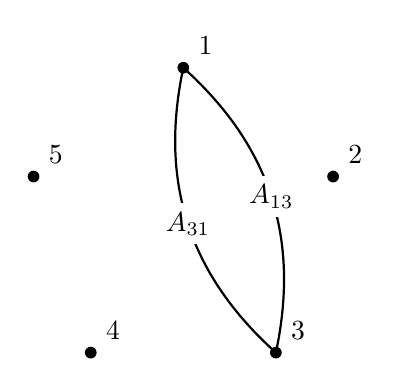
\begin{tikzpicture}

    % Define the radius of the circle and number of dots
    \def\radius{2cm}
    \def\n{5}

    % Draw 5 dots in a circle
    \foreach \i in {1,...,\n}{
        \node[circle,fill,inner sep=1.5pt, label={30:{\i}}] at \dotposition{\i} {};
    }

    % Draw a bendy line from dot 1 to dot 3 using bend left
    \draw[thick, bend left] 
        ({-360/\n * (3 - 1) + 90}:\radius) to 
        node[midway, fill=white] {$A_{31}$} % Label at the midpoint
        ({-360/\n * (1 - 1) + 90}:\radius);

    % Draw a bendy line from dot 3 to dot 1 using bend right
    \draw[thick, bend left] 
        ({-360/\n * (1 - 1) + 90}:\radius) to 
        node[midway, fill=white] {$A_{13}$} % Label at the midpoint
        ({-360/\n * (3 - 1) + 90}:\radius);

\end{tikzpicture}
\end{center}

Let's first look at the case with $A_{ij} A_{jl}$. Here is an example of the term ways to get the term $A_{13} A_{35}$ with $N = 9$:

\begin{center}
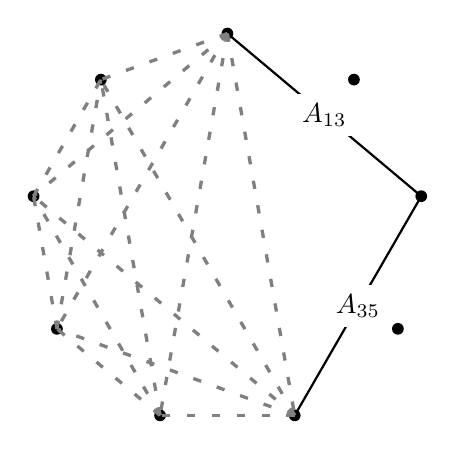
\begin{tikzpicture}

    % Define the radius of the circle and number of dots
    \def\radius{2.5cm}
    \def\n{9}

    % Draw 9 dots in a circle using the macro
    \foreach \i in {1,...,\n}{
        \node[circle,fill,inner sep=1.5pt] at \dotposition{\i} {};
    }

    % Draw a line from dot 1 to dot 3 to dot 5 using the macro
    \draw[thick] 
        \dotposition{1} -- 
        \dotposition{3} node[midway, fill=white] {$A_{13}$} -- 
        \dotposition{5} node[midway, fill=white] {$A_{35}$};

    % Draw grey, more visible dotted lines between dots 5, 6, 7, 8, 9, 1 using the macro
    \foreach \i in {5,6,7,8,9,1}{
        \foreach \j in {5,6,7,8,9,1}{
            \ifnum\i<\j
            \draw[gray, very thick, loosely dashed] \dotposition{\i} -- \dotposition{\j};
            \fi
        }
    }

\end{tikzpicture}
\end{center}

The term can only come from a matrix product involving $\hat{S}_5 D \hat{S}_3 D \hat{S}_1$. Then there is a choice of the other four matrices that can be either $D$ or $\hat{S}_k$.

Choosing a $\hat{S}_k$ matrix will result in a multiplication with a term on the form
\begin{equation}
	2\lambda A_{ij} + 2.
\end{equation}
Since we don't want to add more $A_{ij}$ factors we only care about the multiplication with the $2$. If we choose a $D$ matrix it will flip the sign of the next $2$ term.



\begin{forest}
  for tree={
    circle, draw, minimum size=1.5em, % Style for nodes
    edge={->}, % Arrow for edges
    l sep=20pt, % Space between levels
    s sep=20pt, % Space between siblings
    anchor=center, % Alignment of the tree
  }
  [Root
    [L
      [LL ,edge label={node[midway,left] {2}}
        [LLL, edge label={node[midway,left] {2}}]
        [LLR, edge label={node[midway,right] {-1}}]
	  ]
      [LR
        [LRL, edge label={node[midway,left] {2}}]
        [LRR, edge label={node[midway,right] {-1}}]
      ,edge label={node[midway,right] {-1}}]
    ,edge label={node[midway,left] {2}}]
    [R
      [RL
        [RLL, edge label={node[midway,left] {2}}]
        [RLR, edge label={node[midway,right] {-1}}]
      ,edge label={node[midway,left] {2}}]
      [RR
        [RRL, edge label={node[midway,left] {2}}]
        [RRR, edge label={node[midway,right] {-1}}]
      ,edge label={node[midway,right] {-1}}]
    ,edge label={node[midway,right] {-1}}]
  ]
\end{forest}


We want to show that the constant of motion with factor $\lambda^2$ is equal to the square of the constant of motion with factor $\lambda$ times a constant factor.

We introduce the following notation
\begin{equation}
	A_{ij} = m_i m_j |x_j - x_i|.
\end{equation}

The term with factor $\lambda$ is just the sum
\begin{equation}
	\sum_{1 \leq i < j \leq N} m_i m_j |x_i - x_j|.
\end{equation}
So the term with factor $\lambda^2$ will be
\begin{equation}
\begin{aligned}
	\sum_{i=1}^{N} \sum_{j=1}^{N} &A_{ij}^2 \\
	+2\sum_{i=1}^{N} \sum_{j=1}^{N} \sum_{k=1}^{N} & A_{ij} A_{jk}\\
	+2\sum_{i=1}^{N} \sum_{j=1}^{N} \sum_{k=1}^{N} \sum_{l=1}^{N} & A_{ij} A_{kl}.
\end{aligned}
\end{equation}
with $i \neq j \neq k \neq l$ in all sums. So what we want to show is that for all $N$ the terms on the form $A_{ij} A_{jk}$ and $A_{ij} A_{kl}$ will have a constant coefficient twice as big as the coefficient of $A_{ij}^2$.

So what we want to show is that the terms of $tr(D T_a)$ that have a factor of $\lambda^2$ will be equal to the square of the terms with a factor of $\lambda$ times a constant factor. All terms with a factor of $\lambda^2$ will be of the rorm $\lambda^2 A_{ij} A_{kl}$ and all terms with a factor of $\lambda$ will be of the form $\lambda A_{ij}$. We just need to show that the coefficient of $\lambda^2 A_{ij} A_{kl}, i \neq j \neq k \neq l$, and $\lambda^2 A_{ij} A_{jk}, i \neq j \neq k$ is twice the coefficient of $\lambda A_{ij}^2$.


If we look at all the ways to generate terms on that form we see that it can be represented as a loop on a graph. Every $A_{ij}$ will be an edge between the nodes $i$ and $j$. The edges needs to form a closed loop. All edges will be the factor
\begin{equation}
	2\lambda m_i m_j (x_j - x_i) + 2.
\end{equation}
To get the required factors of $A_{ij}$ only the 

%=========================================================================%
%
% The Appendix
%
%=========================================================================%
\newpage
\appendix

\section{Derivation of the ODE system} \label{sec:DerivationODE}

This section provides proof of that the ODE-system \eqref{eq:peakon_odes} is obtained from the PDE by plugging in the ansatz $u = \sum m_k |x - x_k|$.

\subsubsection*{Preliminaries}

The jump and the average of $f$ at $x_k$ will be defined as
\begin{equation}
	[f(x_k)] := f(x_k^+) - f(x_k^-) \quad \text{and} \quad \langle f(x_k)\rangle := \frac{f(x_k^+) + f(x_k^-)}{2},
\end{equation}
respectively. They satisfy the product rules
\begin{equation} \label{eq:dirac_product_rules}
	[fg] = \langle f\rangle[g] + [f]\langle g\rangle, \quad \quad \langle fg\rangle = \langle f\rangle\langle g\rangle + \frac{1}{4}[f][g].
\end{equation}
%
For a continuous function $f$ and a piecewise continuous function $g$ the product rule for jumps simplifies to
\begin{equation}
	[fg] = f[g].
\end{equation}
In the way the HF-Novikov equation is written here
\begin{equation}
	u_{xxt} = -u^2u_{xxx} - 3uu_xu_{xx},
\end{equation}
there is an issue with term $3uu_xu_{xx}$, since $u_x$ isn't defined at $x_k$ and $u_{xx}$ is a Dirac delta function. One way to get around that is to write the HF-Novikov equation as
\begin{equation}
	-\partial_x^2 u_t - \partial_x^2 u^2 u_x + \partial_x \frac{3}{2} u u_x^2 + \frac{1}{2}u_x^3 = 0.
\end{equation}
%
The first term is 
\begin{equation}
	-\partial_x^2 u_t = - \sum \dot{m}_k 2 \delta_{x_k} + \sum 2 \dot{x}_k m_k \delta'_{x_k}.
\end{equation}
%
The second term $-\partial_x^2 u^2 u_x$ will have the two singular terms
\begin{equation}
	- \sum [(u^2 u_x)_x] \delta_{x_k} - \sum [u^2 u_x] \delta'_{x_k}.
\end{equation}
%
Let's first look at the $\delta'$ term at $x_k$
\begin{equation}
	- [u^2 u_x]_{x_k} = - u^2(x_k) \underbrace{[u_x(x_k)]}_{2m_k} = -2 m_k u^2(x_k).
\end{equation}
Next let's look at the $\delta$ term at $x_k$
\begin{equation}
\begin{aligned}
	- [(u^2 u_x)_x]_{x_k} &= -[2u u_x^2 + u^2 u_{xx}]_{x_k} \\
		&= - 2u(x_k) \underbrace{[u_x^2(x_k)]}_{2\langle u_x \rangle [u_x]}
		- u^2(x_k) \underbrace{[u_{xx}(x_k)]}_{=0} \\
		&= -4u(x_k) \langle u_x(x_k) \rangle \underbrace{[u_x(x_k)]}_{2m_k} = -8m_k u(x_k) u_x(x_k).
\end{aligned}
\end{equation}
The third term $\partial_x \frac{3}{2}u u_x^2$ will have one singular term
\begin{equation}
	\sum [\frac{3}{2} u u_x^2] \delta_{x_k},
\end{equation}
which at $x_k$ will be
\begin{equation}
	[\frac{3}{2}u u_x^2]_{x_k} = \frac{3}{2}u(x_k) \underbrace{[u_x^2(x_k)]}_{2\langle u_x \rangle [u_x]} = 3 \langle u_x(x_k) \rangle \underbrace{[u_x(x_k)]}_{2m_k} = 6m_k u(x_k) u_x(x_k).
\end{equation}
%
The fourth term will not have any singular terms. The $\delta$ and $\delta'$ distributions are linearly independent so the terms can be split up into separate equations. At $x_k$ the sum from all the terms for $\delta$ and $\delta'$ is
\begin{equation}
\begin{aligned}
	0 = -2 \dot{m}_k - [(u^2u_x)_x]_{x_k} + [\frac{3}{2}uu_x^2]_{x_k} = -2 \dot{m}_k - 2 m_k u(x_k) u_x(x_k),
\end{aligned}
\end{equation}
respectively
\begin{equation}
\begin{aligned}
	0 = 2 \dot{x}_k m_k - [u^2u_x]_{x_k} = 2 \dot{x}_k m_k - 2m_ku^2(x_k).
\end{aligned}
\end{equation}
%
The $\dot{m}_k$ equation can be written as
\begin{equation}
	\dot{m}_k = -m_ku_x(x_k)u(x_k).
\end{equation}
It can be assumed that $m_k \neq 0$ since $\dot{m}_k = m_k \cdot (\text{something})$ implies that either $m_k(t) = 0$ for all $t$ or $m_k(t) \neq 0$ for all $t$. If $m_k = 0$ it doesn't contribute anything to $u$ and can therefore be ignored. With $m_k \neq 0$ the expression can be divided by $m_k$ to get
\begin{equation}
	\dot{x}_k = u(x_k)^2.
\end{equation}

The time derivatives you get from periodic ansatz (\refeq{eq:periodic_ansatz}) is of the same form as above. The only difference is that the functions $u(x, t)$ and $u_x(x, t)$ will be the periodic versions of the functions. This is because
\begin{equation}
	u_{xx} = \sum 2 m_k (\delta_x - \delta_{[x_k + L]_{2L}}), 
\end{equation}
so every singular term at $x_k$ will have a corresponding singular term at $[x_k + L]_{2L}$ that will be the same but with a different sign. These terms will give the same form of equations for $\dot{x}_k$ and $\dot{m}_k$ as above.

\section{Verification of the Lax pair for the ansatz}

\todo{Mostly just a copy from the Novikov paper. Is it enough to reference that paper or it good to include again here too?} \\
\todo{Todo: Need to double check that it's correct.}

Generally a function needs to be continuous for the it's multiplication with a Dirac delta function to be well defined. Which creates a problem with the multiplication of $u_x \delta_{x_k}$ since $u_x$ is not continuous at $x_k$. Therefore we will define $u_x \delta_{x_k} := \langle u_x(x_k) \rangle \delta_{x_k}$. The Lax pair formulation is
\begin{equation}
	\partial_x \Psi = \hat{U} \Psi, \qquad \partial_t \Psi = \hat{V} \Psi.
\end{equation}
In this case $\Psi = (\psi_1, \psi_2, \psi_3)^T$ and $\hat{U}$ and $\hat{V}$ are matrices. Both $\hat{U}$ and $\hat{V}$ can be split up into a regular and a singular part
%
\begin{equation}
\hat{U} = U + zmN, \qquad \hat{V} = V - zu^2mN,
\end{equation}
where
\begin{equation}
U =
	\begin{pmatrix}
	0 & 0 & 0 \\
	0 & 0 & 0 \\
	1 & 0 & 0
	\end{pmatrix},
V = 
	\begin{pmatrix}
	-u u_x & \frac{u_x}{z} & u_x^2 \\
	\frac{u}{z} & - \frac{1}{z^2} & - \frac{u_x}{z} \\
	-u^2 & \frac{u}{z} & uu_x
	\end{pmatrix},
N =
	\begin{pmatrix}
	0 & 1 & 0 \\
	0 & 0 & 1 \\
	0 & 0 & 0
	\end{pmatrix}.
\end{equation}
%
We also have that
\begin{equation}
	u = \sum m_k |x - x_k|, \quad u_x = \sum m_k \sgn(x - x_k), \quad m = u_{xx} = \sum 2 m_k \delta(x - x_k).
\end{equation}
Next we do the mixed partials
\begin{equation}
\begin{aligned}
	\partial_t \partial_x \Psi &= \partial_t (U \Psi + zmN \Psi) \\ 
	&= (\underbrace{U_t}_{=0} + U\hat{V}) \Psi + (zm N \Psi)_t \\
	&= UV \Psi - 2zu^2mUN\Psi + 2zN\sum ((m_k \Psi(x_k))_t - m_k \dot{x}_k\Psi(x_k)\dot{x}_k\delta'_{x_k}), \\
	\partial_x \partial_t \Psi &= \partial_t (V \Psi + zu^2mN \Psi) \\
	&= (V_x + VU) \Psi + \sum [ V \Psi ] \delta_{x_k} + 2zN \sum(u(x_k)^2 m_k \Psi(x_k) \delta'_{x_k}).
\end{aligned}
\end{equation}
The mixed partials should be equal. The terms involving $\delta'_{x_k}$ are equal since $\dot{x}_k = u(x_k)^2$. The regular of the mixed partials is
\begin{equation}
	UV - VU - V_x =
	\begin{pmatrix}
		u u_{xx} & -\frac{u_{xx}}{z} & -2 u_x u_{xx} \\
		0 & 0 & \frac{u_{xx}}{z} \\
		0 & 0 & -u u_{xx}
	\end{pmatrix},
\end{equation}
which is identically zero, since the regular part of $u_{xx}$ is zero. Thus the compatibility condition reduces to an equality between the coefficients of $\delta_{x_k}$,
\begin{equation} \label{eq:singular_mixed_partials}
	-2zm_ku(x_k)^2UN\Psi(x_k) + (zmN \Psi(x_k))_t - \sum [V \Psi(x_k)] = 0.
\end{equation}
Using the produce rule (\ref{eq:dirac_product_rules}) and that $[\Psi(x_k)] = 2zm_kN\Psi(x_k)$ we get that
\begin{equation}
\begin{aligned}
	&\sum [V \Psi(x_k)] \delta_{x_k} 
	= \sum \langle V(x_k) \rangle 2zmN\Psi(x_k) + [V(x_k)]\langle \Psi(x_k) \rangle \\
	&= 2zm_k
	\begin{psmallmatrix}
		0 & -u\langle u_x \rangle & \langle u_x \rangle/z \\
		0 & u/z & -1/z^2 \\
		0 & -u^2 & u/z \\
	\end{psmallmatrix}_{x_k} \Psi(x_k)
	+2m_k
	\begin{psmallmatrix}
		u & -1/z & -2\langle u_x \rangle \\
		0 & 0 & 1/z \\
		0 & 0 & -u \\
	\end{psmallmatrix}_{x_k} \langle \Psi(x_k) \rangle.
\end{aligned}
\end{equation}
The $(3,2)$ element $u^2$ in the first term above is going to cancel out the first term in (\ref{eq:singular_mixed_partials}) since $UN$'s only non zero element is the $(3,2)$ element which is one. What's then left of the compatibility condition is
\begin{equation}
\begin{aligned}
	&\dot{m}_k N \Psi(x_k) + m_k N \partial_t \Psi(x_k) \\
	&= m_k
	\begin{psmallmatrix}
		0 & -u\langle u_x \rangle & \langle u_x \rangle/z \\
		0 & u/z & -1/z^2 \\
		0 & 0 & u/z \\
	\end{psmallmatrix}_{x_k} \Psi(x_k)
	+m_k
	\begin{psmallmatrix}
		u & -1/z^2 & -2\langle u_x \rangle/z \\
		0 & 0 & 1/z^2 \\
		0 & 0 & -u/z \\
	\end{psmallmatrix}_{x_k} \langle \Psi(x_k) \rangle.
\end{aligned}
\end{equation}
%
Next let's compute $N \partial_t \langle \Psi(x_k) \rangle$
\begin{equation}
\begin{aligned}
	N \partial_t \langle \Psi(x_k) \rangle 
	&= N (\langle U \Psi(x_k) \rangle \dot{x}_k + \langle V \Psi(x_k) \rangle)\\
	&= N (U u(x_k)^2 \langle A(x_k) \rangle) \langle \Psi(x_k) \rangle + N\frac{1}{4}[A(x_k)][\Psi(x_k)] \\
	&= 
	\begin{psmallmatrix}
		u/z & -1/z^2 & -\langle u_x \rangle/z \\
		0 & u/z & u \langle u_x \rangle \\
		0 & 0 & 0 \\
	\end{psmallmatrix}_{x_k} \langle \Psi(x_k) \rangle
	+\frac{1}{4} \underbrace{N [A(x_k)] N}_{=0} 2z m_k \Psi(x_k).
\end{aligned}
\end{equation}
After a bit of manipulation and using that $\langle \psi_3 \rangle (x_k) = \psi_3(x_k)$, we can show that the compatibility condition can be written as
\begin{equation}
\begin{aligned}
	m_k N \partial_t (\Psi(x_k) - \langle \Psi(x_k) \rangle) + (\dot{m}_k + m_k u(x_k) \langle u_x(x_k) \rangle) N \Psi(x_k) \\
	= m_k \begin{psmallmatrix}
		0 & 0 & 0 \\
		0 & u/z & 0 \\
		0 & 0 & 0
	\end{psmallmatrix}_{x_k} (\Psi(x_k) - \langle \Psi(x_k) \rangle).
\end{aligned}
\end{equation}
The third row is zero and the first two rows says that
\begin{equation}
\begin{aligned}
	(\dot{m}_k + m_ku(x_k) \langle u_x(x_k) \rangle) \psi_2(x_k) &= -m_k \partial_t (\psi_2(x_k) - \langle \psi_2(x_k) \rangle), \\
	(\dot{m}_k + m_ku(x_k) \langle u_x(x_k) \rangle) \psi_3(x_k) &= \frac{1}{z}m_k u(x_k) (\psi_2(x_k) - \langle \psi_2(x_k) \rangle).
\end{aligned}
\end{equation}
If we choose to assign $\psi_2(x_k) = \langle \psi_2(x_k) \rangle$ then it's clear that the compatibility condition is satisfied only if
\begin{equation}
	\dot{m}_k = -m_k u(x_k) \langle u_x(x_k) \rangle.
\end{equation}

%=========================================================================%
%
% Bibliography. The References are added to the file
% references.bib. Use, e.g. \cite{grote:97} to make a reference.
%
%=========================================================================%
\newpage
\bibliographystyle{plain}
\bibliography{references.bib}








\end{document}
